%  ========================================================================
%  Copyright (c) 1995-2012 The University of Washington
%
%  Licensed under the Apache License, Version 2.0 (the "License");
%  you may not use this file except in compliance with the License.
%  You may obtain a copy of the License at
%
%      http://www.apache.org/licenses/LICENSE-2.0
%
%  Unless required by applicable law or agreed to in writing, software
%  distributed under the License is distributed on an "AS IS" BASIS,
%  WITHOUT WARRANTIES OR CONDITIONS OF ANY KIND, either express or implied.
%  See the License for the specific language governing permissions and
%  limitations under the License.
%  ========================================================================
%

% Documentation for UW thesis document style for LaTeX
% by Jim Fox
% fox@washington.edu
%
%    Revised for version 2012/06/19 of uwthesis.cls
%
%    This document is contained in a single file ONLY because
%    I wanted to be able to distribute it easily.  A real thesis ought
%    to be contained on many files (e.g., one for each chapter, at least).
%
%    To help you identify the files and sections in this large file
%    I use the string '==========' to identify new files.
%
%    To help you ignore the unusual things I do with this sample document
%    I try to use the notation
%       
%    % --- sample stuff only -----
%    special stuff for my document, but you don't need it in your thesis
%    % --- end-of-sample-stuff ---


%    Printed in twoside style now that that's allowed
%
 
\documentclass [11pt, twoside] {uwthesis}[2012/06/19]
 
%
% The following line would print the thesis in a postscript font 

% \usepackage{natbib}
% \def\bibpreamble{\protect\addcontentsline{toc}{chapter}{Bibliography}}

\setcounter{tocdepth}{1}  % Print the chapter and sections to the toc
 

% ==========   Local defs and mods
%

% --- sample stuff only -----
% These format the sample code in this document

\usepackage{alltt}  % 
\newenvironment{demo}
  {\begin{alltt}\leftskip3em
     \def\\{\ttfamily\char`\\}%
     \def\{{\ttfamily\char`\{}%
     \def\}{\ttfamily\char`\}}}
  {\end{alltt}}
 
% metafont font.  If logo not available, use the second form
%
% \font\mffont=logosl10 scaled\magstep1
\let\mffont=\sf
% --- end-of-sample-stuff ---
 
\usepackage{epsfig}
\usepackage{graphicx}% Include figure files
\usepackage{dcolumn}% Align table columns on decimal point
\usepackage{bm}% bold math
\usepackage{hyperref}% add hypertext capabilities
\usepackage{amsthm}
\usepackage{amsmath}
\usepackage{amssymb}

\newcommand{\sgn}{\text{sgn}}
\newcommand{\braket}[2]{\langle #1|#2 \rangle}
\newcommand{\normtwo}{\frac{1}{\sqrt{2}}}
\newcommand{\norm}[1]{\parallel #1 \parallel}
\newcommand{\card}[1]{\left| #1 \right|}
\newcommand{\ci}{\perp\!\!\!\perp}
\newtheorem{definition}{Definition}
\newtheorem{lemma}{Lemma}
\newtheorem{theorem}{Theorem}

% To fix Qcircuit target with new Xypic
\newcommand{\targfix}{\qw {\xy {<0em,0em> \ar @{ - } +<.39em,0em>
\ar @{ - } -<.39em,0em> \ar @{ - } +
<0em,.39em> \ar @{ - }
-<0em,.39em>},<0em,0em>*{\rule{.01em}{.01em}}*+<.8em>\frm{o}
\endxy}}

%    Q-circuit version 1.06
%    Copyright (C) 2004  Steve Flammia & Bryan Eastin

%    This program is free software; you can redistribute it and/or modify
%    it under the terms of the GNU General Public License as published by
%    the Free Software Foundation; either version 2 of the License, or
%    (at your option) any later version.
%
%    This program is distributed in the hope that it will be useful,
%    but WITHOUT ANY WARRANTY; without even the implied warranty of
%    MERCHANTABILITY or FITNESS FOR A PARTICULAR PURPOSE.  See the
%    GNU General Public License for more details.
%
%    You should have received a copy of the GNU General Public License
%    along with this program; if not, write to the Free Software
%    Foundation, Inc., 59 Temple Place, Suite 330, Boston, MA  02111-1307  USA

\usepackage[matrix,frame,arrow]{xy}
\usepackage{amsmath}
\newcommand{\bra}[1]{\left\langle{#1}\right\vert}
\newcommand{\ket}[1]{\left\vert{#1}\right\rangle}
    % Defines Dirac notation.
\newcommand{\qw}[1][-1]{\ar @{-} [0,#1]}
    % Defines a wire that connects horizontally.  By default it connects to the object on the left of the current object.
    % WARNING: Wire commands must appear after the gate in any given entry.
\newcommand{\qwx}[1][-1]{\ar @{-} [#1,0]}
    % Defines a wire that connects vertically.  By default it connects to the object above the current object.
    % WARNING: Wire commands must appear after the gate in any given entry.
\newcommand{\cw}[1][-1]{\ar @{=} [0,#1]}
    % Defines a classical wire that connects horizontally.  By default it connects to the object on the left of the current object.
    % WARNING: Wire commands must appear after the gate in any given entry.
\newcommand{\cwx}[1][-1]{\ar @{=} [#1,0]}
    % Defines a classical wire that connects vertically.  By default it connects to the object above the current object.
    % WARNING: Wire commands must appear after the gate in any given entry.
\newcommand{\gate}[1]{*{\xy *+<.6em>{#1};p\save+LU;+RU **\dir{-}\restore\save+RU;+RD **\dir{-}\restore\save+RD;+LD **\dir{-}\restore\POS+LD;+LU **\dir{-}\endxy} \qw}
    % Boxes the argument, making a gate.
\newcommand{\meter}{\gate{\xy *!<0em,1.1em>h\cir<1.1em>{ur_dr},!U-<0em,.4em>;p+<.5em,.9em> **h\dir{-} \POS <-.6em,.4em> *{},<.6em,-.4em> *{} \endxy}}
    % Inserts a measurement meter.
\newcommand{\measure}[1]{*+[F-:<.9em>]{#1} \qw}
    % Inserts a measurement bubble with user defined text.
\newcommand{\measuretab}[1]{*{\xy *+<.6em>{#1};p\save+LU;+RU **\dir{-}\restore\save+RU;+RD **\dir{-}\restore\save+RD;+LD **\dir{-}\restore\save+LD;+LC-<.5em,0em> **\dir{-} \restore\POS+LU;+LC-<.5em,0em> **\dir{-} \endxy} \qw}
    % Inserts a measurement tab with user defined text.
\newcommand{\measureD}[1]{*{\xy*+=+<.5em>{\vphantom{#1}}*\cir{r_l};p\save*!R{#1} \restore\save+UC;+UC-<.5em,0em>*!R{\hphantom{#1}}+L **\dir{-} \restore\save+DC;+DC-<.5em,0em>*!R{\hphantom{#1}}+L **\dir{-} \restore\POS+UC-<.5em,0em>*!R{\hphantom{#1}}+L;+DC-<.5em,0em>*!R{\hphantom{#1}}+L **\dir{-} \endxy} \qw}
    % Inserts a D-shaped measurement gate with user defined text.
\newcommand{\multimeasure}[2]{*+<1em,.9em>{\hphantom{#2}} \qw \POS[0,0].[#1,0];p !C *{#2},p \drop\frm<.9em>{-}}
    % Draws a multiple qubit measurement bubble starting at the current position and spanning #1 additional gates below.
    % #2 gives the label for the gate.
    % You must use an argument of the same width as #2 in \ghost for the wires to connect properly on the lower lines.
\newcommand{\multimeasureD}[2]{*+<1em,.9em>{\hphantom{#2}}\save[0,0].[#1,0];p\save !C *{#2},p+LU+<0em,0em>;+RU+<-.8em,0em> **\dir{-}\restore\save +LD;+LU **\dir{-}\restore\save +LD;+RD-<.8em,0em> **\dir{-} \restore\save +RD+<0em,.8em>;+RU-<0em,.8em> **\dir{-} \restore \POS !UR*!UR{\cir<.9em>{r_d}};!DR*!DR{\cir<.9em>{d_l}}\restore \qw}
    % Draws a multiple qubit D-shaped measurement gate starting at the current position and spanning #1 additional gates below.
    % #2 gives the label for the gate.
    % You must use an argument of the same width as #2 in \ghost for the wires to connect properly on the lower lines.
\newcommand{\control}{*-=-{\bullet}}
    % Inserts an unconnected control.
\newcommand{\controlo}{*!<0em,.04em>-<.07em,.11em>{\xy *=<.45em>[o][F]{}\endxy}}
    % Inserts a unconnected control-on-0.
\newcommand{\ctrl}[1]{\control \qwx[#1] \qw}
    % Inserts a control and connects it to the object #1 wires below.
\newcommand{\ctrlo}[1]{\controlo \qwx[#1] \qw}
    % Inserts a control-on-0 and connects it to the object #1 wires below.
\newcommand{\targ}{*{\xy{<0em,0em>*{} \ar @{ - } +<.4em,0em> \ar @{ - } -<.4em,0em> \ar @{ - } +<0em,.4em> \ar @{ - } -<0em,.4em>},*+<.8em>\frm{o}\endxy} \qw}
    % Inserts a CNOT target.
\newcommand{\qswap}{*=<0em>{\times} \qw}
    % Inserts half a swap gate. 
    % Must be connected to the other swap with \qwx.
\newcommand{\multigate}[2]{*+<1em,.9em>{\hphantom{#2}} \qw \POS[0,0].[#1,0];p !C *{#2},p \save+LU;+RU **\dir{-}\restore\save+RU;+RD **\dir{-}\restore\save+RD;+LD **\dir{-}\restore\save+LD;+LU **\dir{-}\restore}
    % Draws a multiple qubit gate starting at the current position and spanning #1 additional gates below.
    % #2 gives the label for the gate.
    % You must use an argument of the same width as #2 in \ghost for the wires to connect properly on the lower lines.
\newcommand{\ghost}[1]{*+<1em,.9em>{\hphantom{#1}} \qw}
    % Leaves space for \multigate on wires other than the one on which \multigate appears.  Without this command wires will cross your gate.
    % #1 should match the second argument in the corresponding \multigate. 
\newcommand{\push}[1]{*{#1}}
    % Inserts #1, overriding the default that causes entries to have zero size.  This command takes the place of a gate.
    % Like a gate, it must precede any wire commands.
    % \push is useful for forcing columns apart.
    % NOTE: It might be useful to know that a gate is about 1.3 times the height of its contents.  I.e. \gate{M} is 1.3em tall.
    % WARNING: \push must appear before any wire commands and may not appear in an entry with a gate or label.
\newcommand{\gategroup}[6]{\POS"#1,#2"."#3,#2"."#1,#4"."#3,#4"!C*+<#5>\frm{#6}}
    % Constructs a box or bracket enclosing the square block spanning rows #1-#3 and columns=#2-#4.
    % The block is given a margin #5/2, so #5 should be a valid length.
    % #6 can take the following arguments -- or . or _\} or ^\} or \{ or \} or _) or ^) or ( or ) where the first two options yield dashed and
    % dotted boxes respectively, and the last eight options yield bottom, top, left, and right braces of the curly or normal variety.
    % \gategroup can appear at the end of any gate entry, but it's good form to pick one of the corner gates.
    % BUG: \gategroup uses the four corner gates to determine the size of the bounding box.  Other gates may stick out of that box.  See \prop. 
\newcommand{\rstick}[1]{*!L!<-.5em,0em>=<0em>{#1}}
    % Centers the left side of #1 in the cell.  Intended for lining up wire labels.  Note that non-gates have default size zero.
\newcommand{\lstick}[1]{*!R!<.5em,0em>=<0em>{#1}}
    % Centers the right side of #1 in the cell.  Intended for lining up wire labels.  Note that non-gates have default size zero.
\newcommand{\ustick}[1]{*!D!<0em,-.5em>=<0em>{#1}}
    % Centers the bottom of #1 in the cell.  Intended for lining up wire labels.  Note that non-gates have default size zero.
\newcommand{\dstick}[1]{*!U!<0em,.5em>=<0em>{#1}}
    % Centers the top of #1 in the cell.  Intended for lining up wire labels.  Note that non-gates have default size zero.
\newcommand{\Qcircuit}{\xymatrix @*=<0em>}
    % Defines \Qcircuit as an \xymatrix with entries of default size 0em.


\begin{document}
 
% ==========   Preliminary pages
%
% ( revised 2012 for electronic submission )
%

\prelimpages
 
%
% ----- copyright and title pages
%
\Title{Low-depth quantum architectures}
\Author{Paul Pham}
\Year{2013}
\Program{University of Washington Computer Science \& Engineering}

\Chair{Aram Harrow}{Visiting Professor}{Computer Science \& Engineering}
\Signature{Paul Beame}
\Signature{Mark Oskin}
\Signature{Boris Blinov}

\copyrightpage

% \titlepage  

% --- sample stuff only -----
% unusual footnote not found in a real thesis
% You just use the \titlepage as commented out above

{\Degreetext{A dissertation \\
%  \footnote[2]{an egocentric imitation, actually}\\
  submitted in partial fulfillment of the\\ requirements for the degree of}
 \def\thefootnote{\fnsymbol{footnote}}
 \let\footnoterule\relax
 \titlepage
 }
\setcounter{footnote}{0}

% --- end-of-sample-stuff ---
 
%
% ----- signature and quoteslip are gone
%

%
% ----- abstract
%


\setcounter{page}{-1}
\abstract{%

} 
%
% ----- contents & etc.
%
\tableofcontents
\listoffigures
%\listoftables  % I have no tables
 
%
% ----- glossary 
%
\chapter*{Glossary}      % starred form omits the `chapter x'
\addcontentsline{toc}{chapter}{Glossary}
\thispagestyle{plain}
%
\begin{glossary}
\item[quantum architecture] the study of how to lay out quantum bits and their
allowed interactions in a physical system to execute quantum algorithms
efficiently in time, space, and other resources.
 
\end{glossary}
 
%
% ----- acknowledgments
%
\acknowledgments{% \vskip2pc
  % {\narrower\noindent
  This section remains to be written.
    % \par}
}

%
% ----- dedication
%
\dedication{\begin{center}to be decided\end{center}}

%
% end of the preliminary pages
 
 
 
%
% ==========      Text pages
%

\textpages
 
% ========== Chapter 1
\chapter {Shor's Factoring Algorithm on a Nearest-Neighbor Architecture}
\label{chap:factor-polylog}

\section{Abstract}
%%%%%%%%%%%%%%%%%%%%
% put abstract here
%%%%%%%%%%%%%%%%%%%%
We present a 2D nearest-neighbor
quantum architecture for Shor's algorithm to factor an $n$-bit number in $O(\log^3n)$ depth.
Our implementation uses
%(1)
parallel phase estimation,
%(due to Kitaev, Shen, and Vyalyi),
%(2)
constant-depth fanout and teleportation,
%(due to Harrow, Fowler, and Taylor),
and
%(3)
constant-depth carry-save modular addition.
%(due to Gossett).
%We introduce a novel 2D architectural variation on Gossett's modular arithmetic
%and interleave constant-depth fanout and teleportation circuits for
%nearest-neighbor and long-distance communication channels, and ultimately use
%our circuit within parallel phase estimation to achieve quantum factoring.
We derive upper bounds on the circuit resources of our architecture under a
new 2D model which allows a classical controller and parallel, communicating
modules.
We provide a comparison to all previous nearest-neighbor factoring
implementations.  
Our circuit results in an exponential improvement in nearest-neighbor circuit depth at the cost of a polynomial increase in circuit size and width.

\section{Introduction}
\label{sec:fpl-intro}

Shor's factoring algorithm is a central result in quantum computing, with an
exponential speed-up over the best known classical algorithm \cite{Shor1994}.
As the most notable example of a quantum-classical complexity separation, much
effort has been devoted to implementations of factoring on a
realistic architectural model of a quantum computer
\cite{Beauregard2002,Kutin2006,VanMeter2006,VanMeter2005,VanMeterIL2005}.
We can bridge the gap between
the theoretical algorithm and a physical implementation by describing
the layout and interactions of qubits at an intermediate,
architectural level of abstraction.
This gives us a model for measuring circuit resources and their tradeoffs.
In this work, we present a circuit implementation for prime
factorization of an $n$-bit integer
on a two-dimensional architecture that allows concurrent (parallel) two-qubit operations
between neighboring qubits, an omnipresent classical controller, and
modules which are allowed to teleport qubits to each other. We call this new
model \textsc{\textsf{2D CCNTCM}}.
We show that our circuit construction is asymptotically more efficient in circuit depth than previous state-of-the-art techniques for nearest-neighbor
architectures, achieving a depth of $O(\log^3 n)$, a size of
$O(n^4\log n)$, and a width of $O(n^4)$ qubits, as detailed in Table
\ref{tab:fpl-results} of Section \ref{sec:fpl-results}.

Our technique hinges on several key building blocks.
Section \ref{sec:fpl-bg} introduces quantum architectural models, circuit
resources, and constant-depth communication techniques due to
\cite{Harrow2012,Rosenbaum2012}.
Section \ref{sec:fpl-related} places our work in the context of existing
results.
In Section \ref{sec:csa}, we provide a self-contained pedagogical review
of the carry-save technique and encoding.
In Section \ref{sec:csa-mod-add} we modify and extend the carry-save technique to a 2D
modular adder,
which we then use as a basis for a modular multiplier
(Section \ref{sec:csa-mod-mult}) and a modular exponentiator
(Section \ref{sec:modexp}).
For each building block, we provide numerical upper bounds for the
required circuit resources.
Finally, we compare our asymptotic circuit resource usage
with other factoring implementations.


\section{Background}
\label{sec:fpl-bg}

Quantum architecture is the design of physical qubit layouts
and their allowed interactions to execute
quantum algorithms efficiently in time, space, and other
resources.
In this paper, we focus on designing a realistic nearest-neighbor circuit for running
Shor's factoring algorithm on two-dimensional
architectural models of a physical quantum device with nearest-neighbor
interactions.

%%%%%%%%%%%%%%%%%%%%%%%%%%%%%%%%%%%%%%%%%%%%%%%%%%%%%%%%%%%%%%%%%%%%%%%%%%%%%%%
\subsection{Architectural Models and Circuit Resources}
\label{subsec:models}

Following Van Meter and Itoh \cite{VanMeter2005},
we distinguish between a model and an architectural implementation as follows.
A \emph{model} is a set of constraints and rules for the placement and
interaction of qubits.
An \emph{architecture} (or interchangeably, an \emph{implementation} 
or a \emph{circuit}) is a particular
spatial layout of qubits (as a graph of vertices) and allowed interactions (edges between the vertices),
following the constraints of a given model. In this section, we describe
several models which try to incorporate resources of physical interest from
experimental work. We also introduce a new model,
\textsc{2D CCNTCM}, which we will use to analyze our current circuit.

The most general model is called Abstract Concurrent (\textsc{AC})
and allows arbitrary, long-range interactions between any qubits and concurrent
operation of quantum gates.
This corresponds to a complete graph with an edge between every pair of nodes.
It is the model assumed in most quantum algorithms.

A more specialized model restricts interactions to nearest-neighbor, two-qubit,
concurrent gates (\textsc{NTC}) in a regular one-dimensional chain (1D NTC),
which is sometimes called linear nearest-neighbor (\textsc{LNN}).
This corresponds to a line graph. This is a more realistic model than
\textsc{AC}, but correspondingly, circuits in this model may incur greater
resource overheads.

To relieve movement congestion,
we can consider a two-dimensional regular grid
(2D NTC), where each
qubit has four planar neighbors, and 
there is an extra degree of freedom over the 1D model
in which to move data.
In this paper, we extend the \textsc{2D NTC} model in three ways.
The first two extensions are described in Section \ref{subsec:2dccntc},
and the third extension is described in Section \ref{subsec:2dccntcm}.

\subsection{\textsc{2D CCNTC}: Two-Dimensional Nearest-Neighbor Two-Qubit Concurrent Gates with Classical Controller}
\label{subsec:2dccntc}

The first extension allows arbitrary planar graphs
with bounded degree, rather than a regular square lattice.
Namely, we assume qubits lie in a plane and edges are not allowed to intersect.
All qubits are accessible from above
or below by control and measurement apparatus.
Whereas 2D NTC conventionally assumes each qubit
has four neighbors, we consider up to six neighbors in a roughly hexagonal
layout. The edge length in this model is no more than twice the edge length
in a regular 2D NTC lattice. The second extension is the realistic assumption
that classical control (CC) can
access every qubit in parallel, and we do not count these classical
resources in our implementation since they are polynomially bounded. The
classical controllers
correspond to fast digital computers which are
available in actual experiments and are necessary for constant-depth
communication in the next section.

We call an AC or NTC model augmented by these two extensions
\textsc{CCAC} and \textsc{CCNTC}, respectively. Before we describe the
third extension, let us formalize our model for \textsc{2D CCNTC}, with definitions that are (asymptotically) equivalent to those in 
\cite{Rosenbaum2012}.

\begin{definition}
A 2D CCNTC architecture consists of

\begin{itemize}
\item a quantum computer $QC$ which is represented by a planar graph $(V,E)$. A
node $v \in V$ represents a qubit which is acted upon in a circuit, and an
undirected edge $(u,v) \in E$ represents 
an allowed two-qubit interaction between qubits $u,v \in V$. Each node has
degree at most $6$.
\item a universal gate set $\mathcal{G} = \{X, Z, H, T, T^{\dagger}, CNOT, MeasureZ\}$.

\item a deterministic machine (classical controller) $CC$ that applies a sequence
of concurrent gates in each of $D$ timesteps.
\item In timestep $i$, $CC$ applies a set of
gates $G_i = \{g_{i,j} \in \mathcal{G} \}$.
Each $g_{i,j}$ operates in one of the following two ways:
\begin{enumerate}
\item It is a single-qubit gate from $\mathcal{G}$ acting on a single qubit $v_{i,j} \in V$
\item
It is the gate CNOT from $\mathcal{G}$ acting on two qubits $v^{(1)}_{i,j}, v^{(2)}_{i,j} \in V$ where
$(v^{(1)}_{i,j}, v^{(2)}_{i,j}) \in E$
\end{enumerate}
All the $g_{i,j}$ can only operate on
disjoint qubits for a given timestep $i$. We define the support of $G_i$
as $V_i$, the set of all qubits acted upon during timestep $i$.

\begin{equation}
V_i = \bigcup_{j: g_{i,j} \in G_i} v_{i,j} \cup v^{(1)}_{i,j} \cup v^{(2)}_{i,j}
\end{equation}

\end{itemize}
\end{definition}

We can then define the three conventional circuit resources in this model.

\begin{description}
\item[circuit depth ($D$):] the number of concurrent timesteps.
\item[circuit size ($S$):] the total number of non-identity gates applied
from $\mathcal{G}$, equal to $\sum_{i=1}^D |G_i|$.
\item[circuit width ($W$):] the total number of qubits operated upon by
any gate, including inputs, outputs, and ancillae. It is equal to $| \bigcup_{i=1}^D V_i|$.
\end{description}

We observe that the following relationship holds between the circuit resources.
The circuit size is bounded above by
the product of circuit depth and circuit width, since in the worst case,
every qubit is acted upon by a gate for every timestep of a circuit.
The circuit depth is also bounded above by the size, since in the worst case,
every gate is executed serially without any concurrency.

\begin{equation}
D \le S \le D\cdot W
\label{eqn:depth-width}
\end{equation}

The set $\mathcal{G}$ includes measurement in the $Z$ basis, which is
actually not a unitary operation but which may be slower than unitary
operations in actual practice \cite{DiVincenzo2007}.
Therefore we count it in our resource
estimates.
All other gates
in $\mathcal{G}$ form a universal set of unitary
gates \cite{Kitaev2002}.
 In this paper we
will treat the operations in $\mathcal{G}$ as \emph{elementary gates}.
We can also define a Bell basis measurement using operations
from $\mathcal{G}$. A circuit performing this measurement is shown
in Figure \ref{fig:bell-measure} and has depth $4$,
size $4$, and width $2$.

\begin{figure*}[tb!]
\begin{center}
\begin{displaymath}
\begin{array}{ccc}
\Qcircuit @C=1em @R=1em {
& \qw & \multimeasureD{1}{\mbox{Bell}} & \cw & \rstick{j} \\
& \qw & \ghost{\mbox{Bell}}            & \cw & \rstick{k}
}
& \qquad \equiv \qquad &
\Qcircuit @C=1em @R=1em {
& \qw & \ctrl{1} & \qw & \gate{H} & \qw & \meter & \cw & \rstick{j} \\
& \qw & \targfix & \qw & \qw      & \qw & \meter & \cw & \rstick{k}
}
\end{array}
\end{displaymath}
\centerline{}
\fcaption{A circuit for measurement in the Bell state basis.}
\label{fig:bell-measure}
\end{center}\end{figure*}

The third extension to our model, and the most significant, is to consider
multiple disconnected planar graphs, each of which is a 2D CCNTC
architecture. This is described in more detail in the next section.

\subsection{\textsc{2D CCNTCM}: Two-Dimensional Nearest-Neighbor Two-Qubit Concurrent Gates with Classical Controller and Modules}
\label{subsec:2dccntcm}

A single, contiguous
2D lattice which contains an entire quantum architecture which may be prohibitively large to manufacture. In practice,
scalable experiments will probably use many
smaller quantum computers which communicate by means of shared
entanglement \cite{Monroe2012}.
We call these individual machines \emph{modules}, each of
which is a self-contained \textsc{2D CCNTC} lattice. This should not be
confused with the word ``modular'' as in ``modular arithmetic'' or as
referring to the modulus $m$ which we are trying to factor.

We treat these modules
and teleportations between them as nodes and edges, respectively,
in a higher-level planar graph. The teleportations each transmit one qubit
from one module to another, from any location within the source module
to any location within the destination module, making use of the
omnipresent classical controller. The modules can be arbitrarily far
apart physically, but they have bounded-degree connectivity with other
modules, and their edges are planar (they cannot intersect).

A single module can be part of multiple teleportation operations in a single timestep, as long as they involve disjoint qubits within the module.
We justify this assumption in that it is
possible to establish entanglement between multiple
quantum computers
in parallel. We call this new model \textsc{2D CCNTCM},
and we argue that is captures the essential aspects of 2D architectures
without being overly sensitive to the exact geometry of the lattices involved.
An graphic depiction of three modules in \textsc{2D CCNTCM} is shown in
Figure \ref{fig:modules}. Each module contains within it a
\textsc{2D CCNTC} lattice. We can equivalently consider the omnipresent,
single
classical controller as a collection of multiple classical controllers, one
for each module or teleportation operation, which can inter-communicate
classically and share a clock.

\begin{figure}[btp!]
\begin{center}

\includegraphics[width=4in]{./modules.pdf}
\end{center}
\fcaption{Three modules in the \textsc{2D CCNTCM} model}
\label{fig:modules}
\end{figure}

\begin{definition}
A \textsc{2D CCNTCM} architecture consists of

\begin{itemize}
\item a quantum computer $\overline{QC}$ which is represented by a planar graph $(\overline{V},\overline{E})$. A
node $\overline{v} \in \overline{V}$ represents a module, or a graph $(V,E)$
from a \textsc{2D CCNTC} architecture defined previously. It can have
unbounded degree.
An
undirected edge $(\overline{u},\overline{v}) \in \overline{E}$ represents an
allowed teleportation from any qubit in module $\overline{u}$ to
another qubit in module $\overline{v}$.
\item All modules are restricted to be linear in the number of their qubits:
$|V| = \Theta(n)$ for all $(V,E) \in \overline{V}$.
\item a universal gate set $\mathcal{G} = \{X, Z, H, T, T^{\dagger}, CNOT,
MeasureZ\}$
for the qubits \emph{within the same} modules which is the same as for \textsc{2D CCNTC},
and an additional operation $Teleport$ which only operates on qubits
\emph{in
different} modules.
\item a deterministic machine (classical controller) $\overline{CC}$ that applies a sequence
of concurrent gates in each of $D+\overline{D}$ timesteps.
This can be a separate classical controller
for every pair of modules.
\item In timestep $i$, $\overline{CC}$ applies
gates $G_i = \{g_{i,j} : g_{i,j} \in \mathcal{G} \lor g_{i,j} = Teleport \}$.
That is, there are two kinds of timesteps with respect to the kinds of gates
which operate within them.
\begin{enumerate}
\item In the first kind, gates are exclusively from $\mathcal{G}$, and
they operate within modules as described
for \textsc{2D CCNTC} above. We say there are $D$ such timesteps.
\item In the second kind, gates are exclusively $Teleport$ gates between two qubits $v^{(1)}_{i,j} \in \overline{v}_1$ and
$v^{(2)}_{i,j} \in \overline{v}_2$ for
(possibly non-distinct) modules $\overline{v}_1, \overline{v}_2 \in \overline{V}$.
Again, all such qubits much be distinct within a timestep.
We say there are $\overline{D}$ such timesteps.
\end{enumerate}

Again, we define the support of $G_i$
as $V_i$, the set of all qubits acted upon by any $g_{i.j}$, which
includes all the modules.
\begin{equation}
V_i = \bigcup_{j: g_{i,j} \in G_i} v_{i,j} \cup v^{(1)}_{i,j} \cup v^{(2)}_{i,j} 
\end{equation}

\end{itemize}
\end{definition}

We measure the efficiency of a circuit in this new module using not just
the three conventional circuit resources, but with three novel resources
based on modules.

\begin{description}

%, depicted in Figure \ref{fig:resources}:
\item[module depth ($\overline{D}$):] the depth of consecutive teleportations between modules.
\item[module size ($\overline{S}$):] the number of total qubits teleported between any two modules over all timesteps.
\item[module width ($\overline{W}$):] the number of modules whose qubits are
acted upon during any timestep.

\end{description}

%We can make an observation analogous to Equation \ref{eqn:depth-width} but
%for modules in Equation \ref{eqn:module-depth-width}.

%\begin{equation}
%\overline{D} \le \overline{S} \le \overline{D}\cdot \overline{W}
%\label{eqn:module-depth-width}
%\end{equation}

We note the following relationship between circuit width and
module width.

\begin{equation}
W = O(n\overline{W})
\label{eqn:module-width}
\end{equation}

This restriction imposes some locality on our model by constraining it to
nearest-neighbor gates within a linear-sized group of qubits, but allowing
it long-range teleportation to circumvent onerous geometric constraints.
Using the constant-depth communication in Section \ref{sec:cdc}, and for
the specific case of factoring, we
can simulate arbitrary connectivity between modules with only a polynomial
increase in the module size and a constant increase in module depth.

\subsection{Circuit Resource Comparisons}

Counting gates from $\mathcal{G}$ as having unit size and unit depth
is
an overestimate compared to the model in \cite{Kutin2006}, in which a
two-qubit gate has unit size and unit depth and
absorbs the depth and size of any adjacent single-qubit gates. We intend
for this more pessimistic estimate to reflect the practical difficulties
in compiling these gates using a non-Clifford gate in a fault-tolerant way,
such as the $T$ gate or the Toffoli gate
\cite{Fowler2011}.
%However, these difficulties may be mitigated by using
%Toffoli gates directly, which can be fault-tolerantly implemented using
%magic-state distillation according to recent works \cite{Eastin2012,Jones2013a}.

In both our resource counting method and that of \cite{Fowler2004,Kutin2006}, multiple gates acting on disjoint qubits
can occur in parallel during the same timestep. For each building block,
from modular addition to modular multiplication and finally to modular
exponentiation, we provide closed form equations upper-bounding the required circuit
resources as a function of $n$, the size of the modulus $m$ to be factored.
We will use the
term \emph{numerical upper bound} to distinguish these formulae from asymptotic
upper bounds.

It is possible to reduce the numerical constants with more detailed analysis,
which would be important for any physical implementation.
However, we have chosen instead to simplify the number of terms in the formulae
for the current work. We do not intend for these upper bounds to represent
the optimal or final work in this area.

The modular adder in Section \ref{sec:csa-mod-add} and its carry-save
subcomponents only occur within a single module, so we only give their
circuit resources in terms of circuit depth, circuit size, and circuit width. 
For the modular multiplier in
Section \ref{sec:csa-mod-mult} and the modular exponentiator in
Section \ref{sec:modexp}, we also give circuit resources in
terms of module depth, module size, and module width.

%%%%%%%%%%%%%%%%%%%%%%%%%%%%%%%%%%%%%%%%%%%%%%%%%%%%%%%%%%%%%%%%%%%%%%%%%%%%%%%%
\section{Constant-depth Teleportation, Fanout, and Unfanout}
\label{sec:cdc}

Communication, namely the \emph{moving} and \emph{copying} of quantum information, in nearest-neighbor quantum architectures is challenging.
In this section we quote known results for teleportation and
fanout in constant depth while also contributing a novel construction
for unfanout.

The first challenge of moving quantum information from one site to another over
arbitrarily long distances can be addressed by using
%A related problem is how to teleport a qubit an arbitrary distance.
% in an
%architecture through ancillae prepared in some initial state.
the constant-depth teleportation circuit
shown in Figure \ref{fig:cdt} due to Rosenbaum \cite{Rosenbaum2012}, illustrated using standard quantum circuit
notation \cite{Nielsen2000}. This requires the circuit resources shown in
Table \ref{tab:cd-resources}. The depth includes a layer of $H$ gates; a layer of CNOTs; an interleaved layer of Bell basis measurements; and two layers of
Pauli corrections ($X$ and $Z$ for each qubit), occurring concurrently with
resetting the $\ket{j}$ and $\ket{k}$ qubits back to $\ket{0}$.
These correction layers are not shown in the circuit.

\begin{figure*}[tb!]
\begin{center}
\begin{displaymath}
%\begin{array}{ccc}
\Qcircuit @C=1em @R=1em {
\lstick{\ket{\psi}}	& \qw      & \qw      & \qw & \qw & \qw & \qw & \qw                                          & \qw & \qw & \multimeasureD{1}{\mbox{Bell}} & \cw & \rstick{j_1} \\
\lstick{\ket{0}}    & \gate{H} & \ctrl{1} & \qw & \qw & \qw & \qw & \qw                                          & \qw & \qw & \ghost{\mbox{Bell}}            & \cw & \rstick{k_1} \\
\lstick{\ket{0}}    & \qw      & \targfix & \qw & \qw & \qw & \qw & \qw_{Z^{j_1}X^{k_1}\ket{\psi}}               & \qw & \qw & \multimeasureD{1}{\mbox{Bell}} & \cw & \rstick{j_2} \\
\lstick{\ket{0}}    & \gate{H} & \ctrl{1} & \qw & \qw & \qw & \qw & \qw                                          & \qw & \qw & \ghost{\mbox{Bell}}            & \cw & \rstick{k_2} \\
\lstick{\ket{0}}    & \qw      & \targfix & \qw & \qw & \qw & \qw & \qw_{Z^{j_2}Z^{j_1}X^{k_2}X^{k_1}\ket{\psi}} & \qw & \qw & \multimeasureD{1}{\mbox{Bell}} & \cw & \rstick{j_3} \\
\lstick{\ket{0}}    & \gate{H} & \ctrl{1} & \qw & \qw & \qw & \qw & \qw                                          & \qw & \qw & \ghost{\mbox{Bell}}            & \cw & \rstick{k_3} \\
\lstick{\ket{0}}    & \qw      & \targfix & \qw & \qw & \qw & \qw & \qw & \qw_{Z^{j_1}Z^{j_2}Z^{j_3}X^{k_3}X^{k_2}X^{k_1}\ket{\psi}} & \qw & \qw              & \qw & \qw \\
}
\end{displaymath}
\centerline{}
\caption{Constant-depth circuit based on \protect{\cite{Broadbent2007,Browne2009}} for teleportation over $n=5$ qubits \protect{\cite{Rosenbaum2012}}.}
\label{fig:cdt}
\end{center}\end{figure*}

\begin{figure*}[tb!]
\begin{center}
\begin{displaymath}
%& \qquad \qquad \qquad &
\Qcircuit @C=1em @R=1em {
\lstick{\ket{\psi}}	& \qw      & \qw      & \qw & \qw & \qw & \multimeasureD{1}{\mbox{Bell}'} & \cw & \rstick{j_1} \\
\lstick{\ket{0}}    & \gate{H} & \ctrl{1} & \qw & \qw      & \qw & \ghost{\mbox{Bell}'}            & \cw & \rstick{k_1} \\
\lstick{\ket{0}_1}    & \qw      & \targfix & \qw & \ctrl{1} & \qw & \qw      & \qw & \rstick{Z^{j_1}X^{k_1}\ket{\ell}_1}\\
\lstick{\ket{0}}	& \qw      & \qw      & \qw & \targfix & \qw & \multimeasureD{1}{\mbox{Bell}} & \cw & \rstick{j_2} \\
\lstick{\ket{0}}    & \gate{H} & \ctrl{1} & \qw & \qw      & \qw & \ghost{\mbox{Bell}}           & \cw & \rstick{k_2} \\
\lstick{\ket{0}_2}    & \qw      & \targfix & \qw & \ctrl{1} & \qw & \qw      & \qw & \rstick{Z^{j_2}X^{k_2}X^{k_1}\ket{\ell}_2}\\
\lstick{\ket{0}}	& \qw      & \qw      & \qw & \targfix & \qw & \multimeasureD{1}{\mbox{Bell}} & \cw & \rstick{j_3} \\
\lstick{\ket{0}}    & \gate{H} & \ctrl{1} & \qw & \qw      & \qw & \ghost{\mbox{Bell}}           & \cw & \rstick{k_3} \\
\lstick{\ket{0}_3}    & \qw      & \targfix & \qw & \ctrl{1} & \qw & \qw      & \qw & \rstick{Z^{j_3}X^{k_3}X^{k_2} X^{k_1}\ket{\ell}_3}\\
\lstick{\ket{0}_4}	& \qw      & \qw      & \qw & \targfix & \qw & \qw      & \qw & \rstick{X^{k_3}X^{k_2} X^{k_1}\ket{\ell}_4}\\
}
%& & \\
%(a) & & (b)
%\end{array}
\end{displaymath}
\centerline{}
\caption{Constant-depth circuits based on \protect{\cite{Broadbent2007,Browne2009}} for fanout \protect{\cite{Harrow2012}} of one qubit to $n=4$ entangled copies.}
\label{fig:cdf}
\end{center}\end{figure*}

Although general cloning is
impossible \cite{Nielsen2000}, the second challenge of copying information can be addressed by performing an unbounded quantum
fanout operation:
$\ket{x,y_1,\ldots,y_n} \rightarrow \ket{x,y_1\oplus x, \ldots, y_n\oplus x}$.
This is used in our arithmetic circuits when
a single qubit needs to control (be entangled with) a large quantum register
(called a \emph{fanout rail}).
We employ a constant-depth circuit due to insight from
measurement-based quantum computing \cite{Raussendorf2003}
that relies on the creation of an
$n$-qubit cat state \cite{Browne2009} which was communicated to
us by Harrow and Fowler \cite{Harrow2012}.

This circuit requires $O(1)$-depth, $O(n)$-size, and $O(n)$-width. Approximately
two-thirds of the ancillae are reusable and can be reset to $\ket{0}$ after
being measured. Numerical upper bounds are given in Table \ref{tab:cd-resources}.
The constant-depth fanout circuit is shown in Figure \ref{fig:cdf} for the case of fanning out a given single-qubit state
$\ket{\psi} = \alpha\ket{0} + \beta\ket{1}$ to four qubits.
The technique works by creating multiple small
cat states of a fixed size (in this case, three qubits), linking them
together into a larger cat state of unbounded size with Bell basis measurements,
and finally entangling them with the source qubit to be fanned out.
The qubits marked $\ket{\ell}$ are
entangled into the larger fanned out state given in Equation \ref{eqn:cat4}.
The Pauli corrections from the cat state creation are denoted by
$X^{k_2}$, $X^{k_3}$, $Z^{j_2}$ and $Z^{j_3}$ on qubits ending in
states $\ket{\ell}_1$, $\ket{\ell}_2$,
$\ket{\ell}_3$, and $\ket{\ell}_4$. The Pauli corrections
$X^{k_1}$ and $Z^{j_1}$ are from the Bell basis measurement
entangling the cat state with the source qubit (denoted $\text{Bell}'$).
\begin{equation}
Z_1^{j_1}X_1^{k_1}Z_2^{j_2}X_2^{k_2}X_2^{k_1}Z_{3}^{j_3}X_{3}^{k_3}X_{3}^{k_2}X_{3}^{k_1}X_{4}^{k_3}X_{4}^{k_2}X_{4}^{k_1}
\left(\alpha \ket{0}_1\ket{0}_2\ket{0}_3\ket{0}_4 + \beta \ket{1}_1\ket{1}_2\ket{1}_3\ket{1}_4 \right)
\label{eqn:cat4}
\end{equation}
%
The operators $X^k_i$ and $Z^j_{h}$ denote Pauli $X$ and $Z$ operators
on qubits $i$ and $h$, controlled by classical bits $k$ and $j$,
respectively. These corrections are enacted by the classical controller based on
the Bell measurement outcomes (not depicted).
Note the cascading nature of these corrections.
There can be up to
$n-1$ of these $X$ and $Z$
corrections on the same qubit, which can be simplified by the classical
controller to a single $X$ and $Z$ operation and then applied with a circuit of
depth 2 and size 2. Also, given the symmetric nature of the cat state, there
is an alternate set of Pauli corrections which would give the same state and
is of equal size to the corrections given above.

\begin{figure*}[tb!]
\begin{center}
\begin{displaymath}
\Qcircuit @C=1em @R=1em {
& \lstick{\ket{\ell}}	& \qw & \gate{H} & \qw & \ctrl{1} & \qw & \qw      & \qw &  \measureD{Z} & \cw & \rstick{j_1} & \\
& \lstick{\ket{\ell}}	& \qw & \gate{H} & \qw & \targfix & \qw & \ctrl{1} & \qw & \measureD{Z} & \cw & \rstick{j_2} & \\
& \lstick{\ket{\ell}}	& \qw & \gate{H} & \qw & \ctrl{1} & \qw & \targfix & \qw & \measureD{Z} & \cw & \rstick{j_3} & \\
& \lstick{\ket{\ell}}	& \qw & \gate{H} & \qw & \targfix & \qw & \ctrl{1} & \qw & \measureD{Z} & \cw & \rstick{j_4} & \\
& \lstick{\ket{\ell}}	& \qw & \gate{H} & \qw & \ctrl{1} & \qw & \targfix & \qw & \measureD{Z} & \cw & \rstick{j_5} & \\
& \lstick{\ket{\ell}}	& \qw & \gate{H} & \qw & \targfix & \qw & \ctrl{1} & \qw & \measureD{Z} & \cw & \rstick{j_6} & \\
& \lstick{\ket{\ell}}	& \qw & \gate{H} & \qw & \qw      & \qw & \targfix & \qw & \gate{H} & \qw & \rstick{Z^{j_2 \oplus j_4}(\alpha\ket{0} + \beta\ket{1})}
}
\end{displaymath}
\centerline{}
\caption{A novel, constant-depth circuit for unbounded quantum unfanout on
CCNTC, from the $7$-qubit entangled state $\alpha\ket{0}^{\otimes 7} + \beta\ket{1}^{\otimes 7}$ to the
target product state $(\alpha\ket{0} + \beta\ket{1})\otimes\ket{0}^{\otimes 6}$.}
\label{fig:cdu}
\end{center}\end{figure*}

Reversing the fanout is an operation called \emph{unfanout}. Unfanout
takes as input 
the following entangled $n$-qubit state which is the result of a fanout.

\begin{equation}
\normtwo (\ket{0}^{\otimes n} + \ket{1}^{\otimes n})
\label{eqn:fanned-out}
\end{equation}

The output of unfanout, after Pauli corrections, is the product state
consisting of all $\ket{0}$'s except for a single target qubit $\alpha\ket{0} + \beta\ket{1}$, which is in the
same state as the original source qubit of the fanout.

In the model of \cite{Hoyer2002}, the fanout and unfanout were identical, elementary
operations. In CCNTC, the operations are not identical due to
the one-way nature of the measurement and the
constraints of NTC. In Figure \ref{fig:cdu}, we contribute a novel quantum circuit for unbounded quantum
unfanout for $n=7$ in constant depth on 2D CCNTC.
Note that the state in Equation \ref{eqn:fanned-out}
is completely symmetric in that all qubits are
equivalent entangled copies of each other. Therefore, the asymmetry 
of the final target qubit is entirely determined by the unfanout circuit,
which in this case selects the bottom qubit in the figure.

The initial fanned out state lives in a $2$-dimensional subspace. The
round of Hadamard gates increases its dimension to $2^n$, and the two
interleaved layers of CNOTs in a sense ``disentangle'' the qubits from
one another, up to a Pauli $Z$ correction. This correction, on the
final target qubit, is controlled by the parity of the classical measurements
on every ``even'' qubit ($j_2$ and $j_4$ in the figure), excluding the 
next-to-last qubit ($j_6$ in the figure). Each measurement projects the state of the
target qubit
into a subspace with half the dimension, so $n-1$ measurements project
the target qubit into a final $2$-dimensional subspace, which is the
qubit $\alpha\ket{0} + \beta\ket{1}$.

Although the circuit show works for odd $n$, we can easily take into
account even $n$ with an initial CNOT to ``uncopy'' one qubit from its
neighbors. The unfanout circuit in Figure \ref{fig:cdu} is the
functional inverse of the
fanout circuit in 
Figure \ref{fig:cdf}, but it relies on the fanned-out qubits
being teleported back into adjacent positions,
which is only possible in a 2D layout.
The target qubit of unfanout is usually chosen to be in the same location
as the source qubit of the corresponding fanout. 
The resources for unfanout are given in
Table \ref{tab:cd-resources}.

% From Notebook #16, p. 212
% From Notebook #16, p. 66
\begin{table}
\begin{displaymath}
\begin{tabular}{|c|c|c|c|}
\hline
\text{Circuit Name} & \text{Depth} & \text{Size} & \text{Width}\\
\hline
\text{Teleportation from Figure \ref{fig:cdt}} & 7 & 3n + 4 & n+1\\
\hline
\text{Fanout from Figure \ref{fig:cdf}} & 9 & 10n - 9 & 3n-1 \\
\hline
\text{Unfanout} & $ 6 $ & $ 3n+2 $ & $ n$ \\
\hline
\end{tabular}
\end{displaymath}
\centerline{}
\caption{Circuit resources for teleportation, fanout, and unfanout
(consisting of
alternating rounds of constant-depth teleportation and CNOT).}
\label{tab:cd-resources}
\end{table}

From an experimental perspective, it is physically efficient to create
a cat state in trapped ions using the M{\o}lmer-S{\o}rensen gate
\cite{Sorensen2000}\cite{Benhelm2008}. However, the fanout circuit for
the 2D CCNTCM model would still be useful for other technologies, such
as superconducting qubits on a 2D lattice.


%%%%%%%%%%%%%%%%%%%%%%%%%%%%%%%%%%%%%%%%%%%%%%%%%%%%%%%%%%%%%%%%%%%%%%%%%%%%%%
\section{Related Work}
\label{sec:fpl-related}

Our work builds upon ideas in classical digital and reversible logic and their extension to quantum logic.
Any circuit implementation for Shor's algorithm requires a quantum adder.
Gossett proposed a quantum algorithm for addition using classical carry-save techniques to add
in constant-depth and multiply in logarithmic-depth, with a quadratic
cost in qubits (circuit width) \cite{Gossett1998}. The techniques relies on encoded addition, sometimes
called a 3-2 adder, and derives from classical Wallace trees \cite{Wallace1964}.

Takahashi and Kunihiro discovered a linear-depth
and linear-size quantum adder using zero ancillae \cite{Takahashi2005}.
They also developed an adder with tradeoffs between $O(n/d(n))$ ancillae and
$O(d(n))$-depth for $d(n) = \Omega(\log n)$ \cite{Takahashi2009}. 
Their approach assumes unbounded fanout, which had not previously been mapped to a
nearest-neighbor circuit until our present work.

Studies of architectural constraints, namely restriction to a 2D planar layout, 
were experimentally motivated. For example, these layouts correspond
to early ion trap proposals \cite{Kielpinski2002}
and were later analyzed at the level of physical qubits and error correction in the context of Shor's algorithm \cite{Kubi09}.
Choi and Van Meter designed one of the first adders targeted to a 2D architecture 
and showed it runs in $\Theta(\sqrt{n})$-depth on \textsc{2D NTC} \cite{Choi2010}
using $O(n)$-qubits with dedicated, special-purpose areas of a physical
circuit layout.

%Once an adder implementation is chosen, it can be extended 
%To perform modular reduction, modular multiplication, 
%Modular exponentiation, and ultimately
%quantum period finding (QPF), the only quantum part of the factoring algorithm.
Modular exponentiation is a key component of quantum period-finding (QPF),
and its efficiency relies on that of its underlying adder implementation.
Since Shor's algorithm is a probabilistic algorithm, multiple rounds of
QPF are required to amplify success probability arbitrarily close to 1.
It suffices to determine the resources
required for a single round of QPF with a fixed, modest success probability
(in the current work, $3/4$).

The most common approach to QPF performs controlled
modular exponentiation followed by an inverse quantum Fourier transform
(QFT) \cite{Nielsen2000}. We will call this \emph{serial QPF}, which is
used by the following implementations.
%Quantum circuits proposed for factoring on a nearest-neighbor architecture have assumed a serial QPF circuit.

Beauregard \cite{Beauregard2002}
constructs a cubic-depth quantum period-finder using only $2n+3$ qubits on
\textsc{AC}.
It combines the ideas of Draper's transform adder \cite{Draper2000},
Vedral et al.'s modular arithmetic blocks \cite{Vedral1996}, and a
semi-classical QFT.
This approach was subsequently adapted to \textsc{1D NTC} by Fowler, Devitt,
and Hollenberg
\cite{Fowler2004} to achieve resource counts for an $O(n^3)$-depth
quantum period-finder. Kutin \cite{Kutin2006} later improved this using
an idea from Zalka for approximate multipliers to produce a QPF circuit on
\textsc{1D NTC}
in $O(n^2)$-depth. Thus, there is only a constant overhead from
Zalka's own factoring implementation on \textsc{AC}, which also has
quadratic depth \cite{Zalka1998}.
Takahashi and Kunihiro extended their earlier $O(n)$-depth adder to a factoring
circuit in $O(n^3)$-depth with linear width \cite{Takahashi2006}.
Van Meter and Itoh explore many different approaches for serial QPF,
with their lowest achievable depth being $O(n^2\log n)$ with
$O(n^2)$ on \textsc{NTC} \cite{VanMeter2005}. Cleve and Watrous
calculate a factoring circuit depth of $O(\log^3 n)$ and corresponding
circuit size of $O(n^3)$ on \textsc{AC},
assuming an adder which has depth $O(\log n)$ and
$O(n)$ size and width. We beat this depth and provide a concrete
architectural implementation using an adder with $O(1)$-depth and $O(n)$
size and width.

In the current work, we assume that errors do not affect the storage of qubits
during the circuit's operation. An alternate approach is taken by
Miquel \cite{Miquel1996} and Garcia-Mata \cite{GarciaMata2007}, who both
numerically simulate Shor's algorithm for factoring specific
numbers to determine its sensitivity to errors. Beckman et al. provide a
concrete factoring implementation in ion traps with $O(n^3)$ depth and size and
$O(n)$ width \cite{Beckman1996}.

In all the previous works,
it is assumed that qubits are expensive (width) and that
execution time (depth) is not the limiting constraint.
We make the alternative assumption that ancillae are cheap and that fast classical control
is available which allows access to all qubits in parallel.
Therefore, we optimize circuit depth at the expense of width.
We compare our work primarily to Kutin's method \cite{Kutin2006}.

These works also rely on serial QPF which in turn relies on an inverse QFT.
On an AC architecture, even when approximating the (inverse) QFT by truncating two-qubit
$\pi/2^k$ rotations beyond $k = O(\log n)$, 
the depth is $O(n \log n)$ to factor an $n$-bit number.
To be implemented fault-tolerantly on a quantum device, rotations in the QFT must then be compiled into a discrete gate basis.
This requires at least a $O(\log(1/\epsilon))$ overhead in depth to approximate a rotation with precision $\epsilon$ \cite{Harrow02, Kitaev2002}.
We would like to avoid the use of a QFT due to its compilation overhead.

There is an alternative, parallel version of phase estimation 
\cite{Cleve2000,Kitaev2002}, which we call \emph{parallel QPF} (we refer the reader to Section 13 of \cite{Kitaev2002} for details), which decreases depth in exchange
for increased width and additional classical post-processing.
This eliminates the need to do an inverse QFT.
%We refer the reader to \cite{Kitaev2002} 
%and \cite{Pham2011b} 
%for details.
We develop a nearest-neighbor factoring circuit based on parallel QPF and our proposed 2D quantum arithmetic circuits.
We show that it is asymptotically more efficient than the serial QPF method. 
We compare the circuit resources required by our work with existing serial QPF implementations in Table
\ref{tab:fpl-results} of Section \ref{sec:fpl-results}.
However, a recent result by \cite{Jones2013} allows one to enact a
QFT using only Clifford gates and a Toffoli gate in $O(\log^2 n)$ expected depth.
This would allow us to
greatly improve the constants in our circuit resource upper bounds in Section \ref{sec:modexp} by combining a QFT with parallel multiplication similar to
the approach described in \cite{VanMeter2005,Cleve2000}.


We also note that recent results by Browne, Kashefi, and Perdrix (BKP) connect the power of
measurement-based quantum computing to the quantum circuit model augmented with
unbounded fanout \cite{Browne2009}. Their model, which we adapt and call
\textsc{CCNTC}, uses the classical controller mentioned in Section \ref{sec:cdc}.
Using results by H{\o}yer and {\v S}palek \cite{Hoyer2002} that
unbounded quantum fanout would allow for a constant-depth factoring algorithm,
they conclude that a probabilistic polytime classical machine with access
to a constant-depth one-way quantum computer would also be able to factor
efficiently.

\section{The Constant-Depth Carry-Save Technique}
\label{sec:csa}

Our 2D factoring approach rests on the central technique of the constant-depth
carry-save adder (CSA) \cite{Gossett1998}, which converts the sum of three
numbers $a$, $b$, and $c$, to the sum of two numbers $u$ and $v$:
%\begin{equation}
$a+b+c = u+v$. The explanation of this technique and how it achieves constant depth requires the following definitions.
%\end{equation}

A \emph{conventional number} $x$ can be represented in $n$ bits as
%\begin{equation}
$x = \sum_{i=0}^{n-1} 2^i x_i$,
%\end{equation}
where $x_i \in \{0,1\}$ denotes the $i$-th bit of $x$, which we call
an $i$-bit and has significance $2^i$, and the $0$-th bit is the low-order bit.\footnote{It will be clear from the context whether we mean an
$i$-bit, which has significance $2^i$, or an $i$-bit number.}
Equivalently, $x$ can be represented as a (non-unique)
sum of two smaller, $(n-1)$-bit, conventional numbers, $u$ and $v$.
We say $(u+v)$ is a \emph{carry-save encoded}, or CSE, number.
The CSE representation of an $n$-bit conventional number
consists of $2n-2$ individual
bits where $v_0$ is always $0$ by convention.

Consider a CSA operating on three bits instead of three numbers; 
then a CSA converts the sum of three
$i$-bits into the sum of an $i$-bit (the \emph{sum} bit) and an $(i+1)$-bit
(the \emph{carry} bit):
%\begin{equation}
%\label{eqn:csa-3-2}
$a_i+b_i+c_i = u_i+v_{i+1}$.
%\end{equation}
By convention, the bit $u_i$ is the parity of the input bits
($u_i = a_i \oplus b_i \oplus c_i$) and
the bit $v_{i+1}$ is the majority of $\{a_i, b_i, c_i\}$.
Figure \ref{fig:csa-encoding} gives a concrete example, where
$(u+v)$ has $2n-2 = 8$ bits, not counting $v_0$.

%
It will also be useful to refer to a subset of the bits in a conventional
number using subscripts to indicate a range of indices:
\begin{equation}
x_{(j,k)} \equiv \sum_{i=j}^k 2^ix_i \qquad
x_{(i)} \equiv x_{(i,i)} = 2^ix_i.
\end{equation}
%
Using this notation, the following identity holds:
\begin{equation}
x_{(j,k)} = x_{(j,\ell)} + x_{(\ell+1,k)}, \qquad \text{ for all } j \le \ell < k.
\end{equation}
%
We can express the relationship between the bits of $x$ and $(u+v)$ as follows:
%
\begin{equation}
x = x_{(0,n-1)} \equiv u+v = u_{(0,n-2)} + v_{(1,n-1)}.
\end{equation}
%
Finally, we denote arithmetic modulo $m$ with square brackets.

\begin{equation}
x_{(j,k)} \bmod m = x_{(j,k)}[m]
\end{equation}

\begin{center}
\begin{figure*}[tb!]
\begin{displaymath}
x = 30 = u+v = 8 + 22 = \left\{
\begin{array}{ccccc}
    & u_3 & u_2 & u_1 & u_0 \\
v_4 & v_3 & v_2 & v_1 &    \\
\hline
x_4 & x_3 & x_2 & x_1 & x_0
\end{array}
\right\}
=
\left\{
\begin{array}{ccccc}
    & 1 & 0 & 0 & 0 \\
  1 & 0 & 1 & 1 &   \\
\hline
1 & 1 & 1 & 1 & 0
\end{array}
\right\}
\end{displaymath}
\fcaption{An example of carry-save encoding for the 5-bit conventional number 30.}
\label{fig:csa-encoding}
\end{figure*}
\end{center}
%

\begin{figure}[tb!]
\begin{center}
\begin{displaymath}
\centerline{
\Qcircuit @C=2em @R=2em {
\lstick{\ket{0}}   & \qw      & \qw & \qw                        & \qw & \qw                        & \targfix  & \qw & \qw_{\ket{a_i \wedge (b_i \oplus c_i)}} & \targfix  & \qw       & \qw       & \qw_{\ket{(b_i \wedge c_i) \oplus a_i \wedge (b_i \oplus c_i)}} & \qw & \qswap      & \qswap      & \qw & \rstick{\ket{u_i}} \\
\lstick{\ket{a_i}} & \qw      & \qw & \qw                        & \qw & \qw                        & \ctrl{-1} & \qw & \qw                                     & \qw       & \targfix  & \qw       & \qw_{\ket{a_i \oplus b_i \oplus c_i}}                           & \qw & \qw \qwx    & \qswap \qwx & \qw & \rstick{\ket{0}} \\
\lstick{\ket{b_i}} & \ctrl{1} & \qw & \targfix                   & \qw & \qw_{\ket{b_i \oplus c_i}} & \ctrl{-1} & \qw & \qw                                     & \qw       & \ctrl{-1} & \targfix  & \ctrl{1}                                                        & \qw & \qw \qwx    & \qw         & \qw & \rstick{\ket{b_i}} \\
\lstick{\ket{c_i}} & \ctrl{1} & \qw & \ctrl{-1}                  & \qw & \qw                        & \qw       & \qw & \qw                                     & \qw       & \qw       & \ctrl{-1} & \ctrl{1}                                                        & \qw & \qw \qwx    & \qw         & \qw & \rstick{\ket{c_i}} \\
\lstick{\ket{0}}   & \targfix & \qw & \qw_{\ket{b_i \wedge c_i}} & \qw & \qw                        & \qw       & \qw & \qw                                     & \ctrl{-4} & \qw       & \qw       & \targfix                                                        & \qw & \qswap \qwx & \qw         & \qw & \rstick{\ket{v_{i+1}}}}
}
\end{displaymath}
\fcaption{Carry-save adder circuit for a single bit position $i$: $a_i+b_i+c_i = u_i + v_{i+1}$.}
\label{fig:csa-circuit}
\end{center}\end{figure}

\begin{figure}
\begin{center}
\begin{displaymath}
\begin{tabular}{p{0.5in} m{0.1in} p{2in}}

\Qcircuit @C=1em @R=2.2em { 
	& \qw & \ctrl{1} & \qw & \qw \\
	& \qw & \ctrl{1} & \qw & \qw \\
	& \qw & \targfix & \qw & \qw
}

&
\qquad
=
\qquad
&

\Qcircuit @C=1em @R=.7em { 
	& \gate{T^{\dagger}} & \qw & \targfix  & \qw & \gate{T} & \qw & \targfix  & \qw & \gate{T^{\dagger}} & \qw & \targfix  & \qw & \gate{T}           & \qw & \targfix  & \qw & \qw \\ 
	& \gate{T^{\dagger}} & \qw & \qw       & \qw & \ctrl{1} & \qw & \ctrl{-1} & \qw & \ctrl{1}           & \qw & \qw       & \qw & \qw                & \qw & \ctrl{-1} & \qw & \qw \\
	& \gate{H}           & \qw & \ctrl{-2} & \qw & \targfix & \qw & \gate{T}  & \qw & \targfix           & \qw & \ctrl{-2} & \qw & \gate{T^{\dagger}} & \qw & \gate{H}  & \qw & \qw
}
\end{tabular}
\end{displaymath}
\fcaption{The depth-efficient Toffoli gate decomposition from \cite{Amy2012}.}
\label{fig:toffoli}
\end{center}
\end{figure}

% From Notebook #16, pp. 68-69
\begin{table}
\begin{displaymath}
\begin{tabular}{|c|c|c|c|}
\hline
\text{Circuit Name} & \text{Depth} & \text{Size} & \text{Width} \\
\hline
\text{Toffoli gate from \cite{Amy2012}} and Figure \ref{fig:toffoli} & 8 & 15 & 3 \\
\hline
\text{Single-bit } 3\text{-to-}2 \text{ adder from Figure \ref{fig:csa-circuit}} & 33 & 55 & 5 \\
%\hline
%$n$ \text{-bit modular } 3\text{-to-}2 \text{ adder from Figure \ref{fig:csa-add-4}} & 356 & 572n + 724 & 33n+47 \\
\hline
\end{tabular}
\end{displaymath}
\centerline{}
\tcaption{Circuit resources for Toffoli and single-bit addition.}
\label{tab:csa-tile-resources}
\end{table}

Figure \ref{fig:csa-circuit} gives a circuit description of carry-save addition (CSA) for a single bit position $i$.
The resources for this circuit are given in Table \ref{tab:csa-tile-resources}, using
the resources for the Toffoli gate (in the same table) based on
\cite{Amy2012}. We note here
that a more efficient decomposition for the Toffoli is possible using a
distillation approach described in \cite{Jones2013a}.

We must lay out the circuit to satisfy a 2D NTC model.
The Toffoli gate decomposition in \cite{Amy2012}, duplicated in
Figure \ref{fig:toffoli}, requires two control
qubits and a single target qubit to be
mutually connected to each other. Given this constraint, and the
interaction of the CNOTs in Figure \ref{fig:csa-circuit}, we can
rearrange these qubits on a 2D planar grid and obtain the layout shown
in Figure \ref{fig:csa-3-2}, which satisfies our 2D NTC model.
Qubits $\ket a_i$, $\ket b_i$, and $\ket c_i$ reside at the top of Figure~\ref{fig:csa-3-2}, while qubits $\ket{u_i}$ and $\ket{v_{i+1}}$ are initialized to $\ket 0$.
Upon completion of the circuit, qubit $\ket{a_i}$ is in state $\ket 0$, as seen from the output in Figure~\ref{fig:csa-circuit}. 
Note that this construction uses more gates and one more ancilla than the equivalent
quantum full adder circuit in Figure 5 of \cite{Gossett1998}. However this
is necessary in order to meet our architectural constraints and does not change the
asymptotic results.
Also in Figure \ref{fig:csa-3-2}
is a variation called a 2-2 adder, which simply re-encodes two $i$-bits
into an $i$-bit and an $(i+1)$-bit. The 2-2 adder uses at most the resources
of a 3-2 adder, so we can count it as such in our calculations.
It will be useful in the next section.

\begin{figure}[b!]
\begin{center}
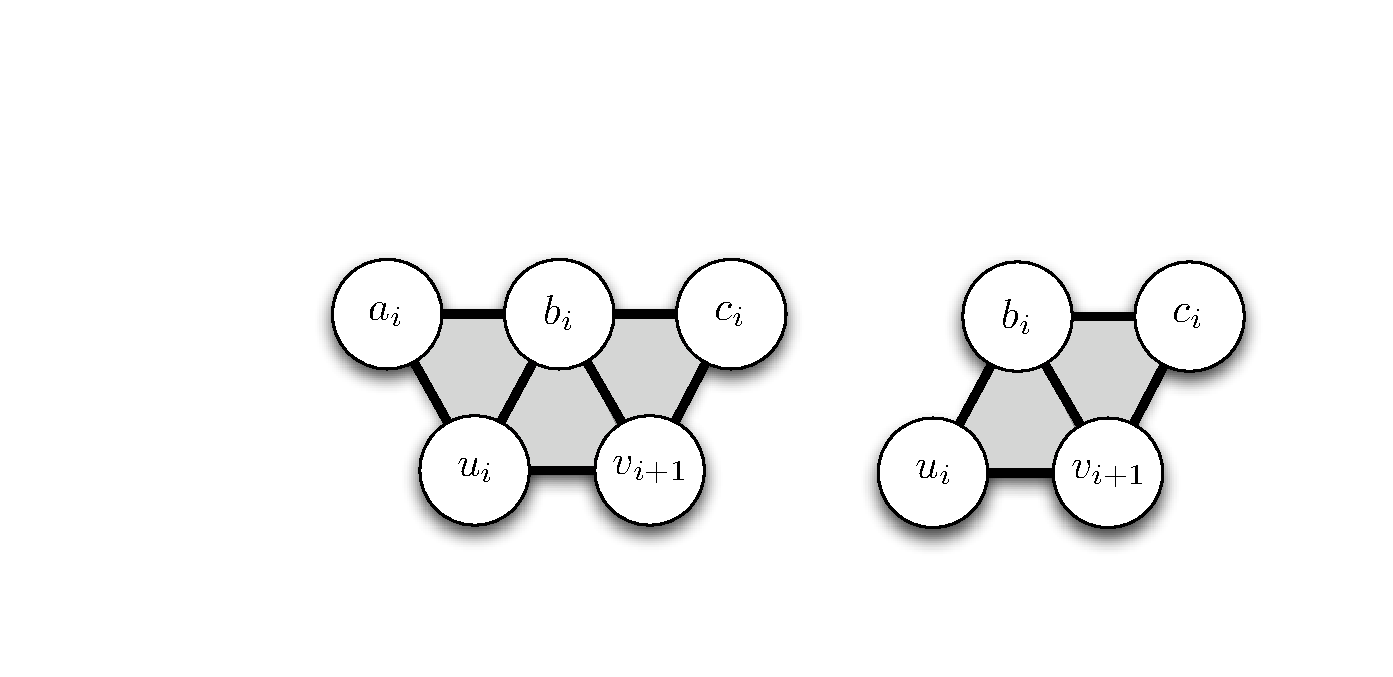
\includegraphics[width=3in]{./csa-32-22.pdf}
\end{center}
\fcaption{The carry-save adder (CSA), or 3-2 adder, and carry-save 2-2 adder.}
\label{fig:csa-3-2}
\end{figure}

At the level of numbers, the sum of three $n$-bit numbers can be converted into
the sum of two $n$-bit numbers by applying a \emph{CSA layer} of
$n$ parallel, single-bit
CSA circuits (Fig.~\ref{fig:csa-circuit}). Since each CSA operates in constant depth, the entire layer also
operates in constant depth, and we have achieved (non-modular) addition.
%
%An important consideration is the circuit width. The circuit above
%requires two additional qubits to contain the output
%out-of-place and produces two garbage qubits: the original inputs
%$b_i$ and $c_i$. 
Each single addition of three $n$-bit numbers requires $O(n)$ circuit width.

\section{Quantum Modular Addition}
\label{sec:csa-mod-add}

To perform addition of two numbers $a$ and $b$ modulo $m$,
we consider the variant problem of modular addition of three numbers to
two numbers:
%
%\begin{quote}
Given three $n$-bit input numbers $a$, $b$, and $c$, and an $n$-bit modulus $m$,
compute
%\begin{equation}
$(u+v) = (a+b+c)[m]$,
%\end{equation}
where $(u+v)$ is a CSE number.

In this section, we provide an alternate, pedagogical explanation of
Gossett's modular reduction \cite{Gossett1998}. Later, we contribute a mapping of this adder
to a 2D architecture,
using unbounded fanout to maintain constant depth for adding back
modular residues. This last step is absent in Gossett's original approach.

To start, we will demonstrate the basic method of modular addition and reduction
on an $n$-bit conventional number. In general, adding two $n$-bit conventional
numbers will produce an overflow bit of significance $2^n$, which we can truncate as long as
we add back its modular residue $2^n \bmod m$. How can we guarantee that we won't
generate another overflow bit by adding back the modular residue? It turns out
we can accomplish this by allowing
a slightly larger input and output number ($n+1$ bits in this case), truncating
multiple overflow bits, and adding back their $n$-bit modular residues.

For two $(n+1)$-bit conventional numbers $x$ and $y$,
we truncate the three high-order bits of their sum $z_{n-1,n+3}$
and
add back their modular residue $x_{(n-1,n)}[m]$:
%
\begin{eqnarray}
x + y \bmod m &=& z_{(0,n+1)}[m] \nonumber \\
&=& z_{(0,n-2)} + z_{(n-1,n+1)}[m].
\end{eqnarray}
%
Since both the truncated number $z_{(0,n-2)}$ and the modular residue
are $n$-bit numbers, their sum is an $(n+1)$-bit number as desired, equivalent
to $x[m]$.

Now we must do the same modular reduction on a CSE number $(u+v)$,
which in this case represents an $(n+2)$-bit conventional number and has
$2n+3$ bits.
%This is the special case mentioned in the
%previous
%section \label{star:csa-special}, where $x$ is the result of a single
%CSA layer, not repeated CSA layers alternating with truncation.
%
%Assume for now that this modular reduction works;
%in the next section we walk through an illustrated concrete example.
%We present a more formal argument in Section \ref{subsec:mod-reduce-1}.
%
First, we truncate the three high-order bits ($v_{n}, u_{n-1}, v_{n-1}$)
of $(u+v)$, yielding an $n$-bit
conventional number with a CSE representation of $2n$ bits:
$\{u_0, u_1, \ldots, u_{n-1}\} \cup \{v_1, v_2, \ldots, v_{n-1}\}$.
Then we add back the three modular residues
$(v_{(n+1)}[m], u_{(n)}[m], v_{(n)}[m])$, and we are guaranteed not to
generate additional overflow bits (of significance $2^{n}$ or higher). This equivalence
is shown in Equation \ref{eqn:mod-reduce}.
\begin{eqnarray}
(u+v)[m] &=& \left(u_{(0,n+1)} + v_{(1,n+2)}\right)[m] \nonumber \\
 &=& u_{(0,n)} +
     v_{(1,n)} + \nonumber \\
 & & u_{(n+1)}[m] +
     v_{(n+1)}[m] + v_{(n+2)}[m]
\label{eqn:mod-reduce}
\end{eqnarray}

\begin{lemma}[Modular Reduction in Constant Depth]
The modular addition of three $n$-bit numbers to two $n$-bit numbers can be
accomplished
in constant depth with $O(n)$ width in \textsc{2D CCNTC}.
\end{lemma}

\begin{proof}
Our goal is to show how to perform modular addition while keeping our numbers
of a fixed size by treating overflow bits correctly.
We map the proof of \cite{Gossett1998} to \textsc{2D CCNTC} and show that
we meet our required depth and width.
First, we enlarge our registers to allow the addition of $(n+2)$-bit numbers,
while keeping our modulus of size $n$ bits.
(In Gossett's original approach, he takes the equivalent step of restricting
the modulus to be of size $(n-2)$ bits.) We accomplish the modular addition
by first performing a layer of non-modular addition, truncating the three high-order
overflow bits, and then adding back modular residues controlled on these
bits in three successive layers, where we are guaranteed that no additional
overflow bits are generated in each layer.
This is illustrated for a $3$-bit modulus and $5$-bit registers
in Figure \ref{fig:csa-proof}.

\begin{center}
\begin{figure*}[h!tb]
\begin{displaymath}
\renewcommand\arraystretch{1.5}
\begin{array}{ccccccll}
        & a_4 & a_3 & a_2 & a_1 & a_0 & 5\text{-bit input number } a &\\
        & b_4 & b_3 & b_2 & b_1 & b_0 & 5\text{-bit input number } b & \\
        & c_4 & c_3 & c_2 & c_1 & c_0 & 5\text{-bit input number } c & \text{[Layer 1]}\\
\hline
        & u_4 & u_3 & u_2 & u_1 & u_0 & \text{truncate } u_{4} & \\
    v_5 & v_4 & v_3 & v_2 & v_1 &     & \text{truncate } v_{4},v_{5} & \\
        &     &     & c^{v_4}_2 & c^{v_4}_1 & c^{v_4}_0 & \text{add back } 2^4 \bmod m \text{ controlled on } v_4 & \text{[Layer 2]}\\
\hline
        &      & u'_3 & u'_2 & u'_1 & u'_0 & & \\
        & v'_4 & v'_3 & v'_2 & v'_1 &      & & \\
        &      &    & c^{u_4}_2 & c^{u_4}_1 & c^{u_4}_0  & \text{add back } 2^4 \bmod m \text{ controlled on } u_4 & \text{[Layer 3]}\\
\hline
        & u''_4 & u''_3 & u''_2 & u''_1 & u''_0 & \text{the bit } u''_4 \text{ is the same as } v'_4 & \\
        & v''_4 & v''_3 & v''_2 & v''_1 &       &  & \\
        &       &    & c^{v_5}_2 & c^{v_5}_1 & c^{v_5}_0 & \text{add back } 2^5 \bmod m \text{ controlled on } v_5 & \text{[Layer 4]}\\
\hline
        & u'''_4 & u'''_3 & u'''_2 & u'''_1 & u'''_0 & \text{ Final CSE output with } 5 \text{ bits} &\\
        & v'''_4 & v'''_3 & v'''_2 & v'''_1 &        & \text{ Final CSE output with } 5 \text{ bits} & \\
\end{array}
%\begin{array}{cccccccr}
%        & a_{n+1} & a_{n} & a_{n-1} & \ldots & a_1 & a_0 & \text{input number } a\\
%        & b_{n+1} & b_{n} & b_{n-1} & \ldots & b_1 & b_0 & \text{input number } b\\
%        & c_{n+1} & c_{n} & c_{n-1} & \ldots & c_1 & c_0 & \text{input number } c\\
%\hline
%        & u_{n+1} & u_{n} & u_{n-1} & \ldots & u_1 & u_0 & \text{truncate } u_{n+1} \\
%v_{n+2} & v_{n+1} & v_{n} & v_{n-1} & \ldots & v_1 & 0   & \text{truncate } v_{n+1},v_{n+2} \\
%        &         &       & x_{n-1} & \ldots & x_1 & x_0 \\
%\hline
%        &         & u'_{n} & u'_{n-1} & \ldots & u'_1 & u'_0 & \\
%        & v'_{n+1} & v'_{n} & v'_{n-1} & \ldots & v'_1 & 0 &  \\
%        &         &       & x_{n-1} & \ldots & x_1 & x_0 \\
%\hline
%        & u''_{n+1} & u''_{n} & u''_{n-1} & \ldots & u''_1 & u''_0 & \\
%        & v''_{n+1} & v''_{n} & v''_{n-1} & \ldots & v''_1 & 0 &  \\
%        &         &       & y_{n-1} & \ldots & y_1 & y_0 \\
%\hline
%        & u'''_{n+1} & u'''_{n} & u'''_{n-1} & \ldots & u'''_1 & u'''_0 & \\
%        & v'''_{n+1} & v'''_{n} & v'''_{n-1} & \ldots & v'''_1 & 0 &  \\
%\hline
%\end{array}
\end{displaymath}
\caption{A schematic proof of Gossett's constant-depth modular reduction for $n=3$.}
\label{fig:csa-proof}
\end{figure*}
\end{center}

We use the following notation.
The non-modular sum of the first layer is $u$ and $v$.
The CSE output of the first modular reduction layer
is $u'$ and $v'$, and the modular residue is
written as $c^{v_{n+1}}$ to mean the precomputed value $2^{n+1} \bmod m$
controlled on $v_{n+1}$.
The CSE output of the second modular reduction layer
is $u''$ and $v''$, and the modular residue is written as
$c^{u_{n+1}}$ to mean the precomputed value $2^{n+1} \bmod m$
controlled on $u_{n+1}$.
The CSE output of the third and final modular reduction layer
is $u'''$ and $v'''$, and the modular residue is written as
$c^{v_{n+2}}$ to mean the precomputed value $2^{n+2} \bmod m$
controlled on $v_{n+2}$.

We show that no layer generates an overflow $(n+2)$-bit, namely in the
$v$ component of any CSE output. (The $u$ component will never exceed the
size of the input numbers.) First, we know that no $v'_{n+2}$ bit
is generated after the first modular reduction layer, because we have
truncated away all $(n+1)$-bits. Second, we know that no $v''_{n+2}$ bit is
generated because we only have one $(n+1)$-bit to add, $v'_{n+1}$.
Finally, we need to show that $v'''_{n+2} = 0$ in the third modular reduction
layer. 

Since $u'_{(n)} + v'_{(n+1)} =
u_{(n)} + v_{(n)} \le 2^{n+1}$, the bits $u'_n$ and $v'_{n+1}$ cannot both be $1$.
But $u''_{n+1} = v'_{n+1}$ and $v''_{n+1} = u'_n\land v'_n$, so $u''_{n+1}$ and
$v''_{n+1}$ cannot both be $1$, and hence $v'''_{n+2} = 0$.
%This bit is the majority of
%$u''_{n+1}$, $v''_{n+1}$, and $c^{v_{n+2}}_{n+1} = 0$. This means we only have
%to guarantee that at most one of $u''_{n+1}$ and $v''_{n+1}$ has value 1.
%This is equivalent to requiring that
%$u''_{(n,n+1)} + v''_{(n+1)} \le 3\cdot 2^{n}$, that is, the sum of these
%three bits has value at most $3$. Bit $u''_{n+1}$ is copied directly from
%$v'_{n+1}$ by the rules of CSA, which requires the following condition for
%the second modular reduction layer:
%$u'_{(n)} + v'_{(n,n+1)} \le 3\cdot 2^n$. This is true because
%$u'_{(n)} + v'_{(n+1)} = u_{(n)} + v_{(n)} \le 2$ and $v'_{(n)} \le 1$.
Everywhere
we use the fact that the modular residues are restricted to $n$ bits.
Therefore, the modular sum is computed as the sum of two $(n+2)$-bit numbers
with no overflows in constant-depth.
\end{proof}

As a side note, we can perform modular reduction in one layer instead of
three by decoding the three overflow bits into one of seven different
modular residues. This can also be done in constant depth, and in this case
we only need to enlarge all our registers to $(n+1)$ bits instead of $(n+2)$
as in the proof above. We omit the proof for brevity.

In the following two subsections, we give a concrete example to illustrate
the modular addition circuit as well as a numerical upper bound for the
general circuit resources.

%%%%%%%%%%%%%%%%%%%%%%%%%%%%%%%%%%%%%%%%%%%%%%%%%%%%%%%%%%%%%%%%%%%%%%%%%%%%%%%
\subsection{A Concrete Example of Modular Addition}
\label{subsec:concrete}

\begin{center}
\begin{figure*}[h!bt]
\centerline{
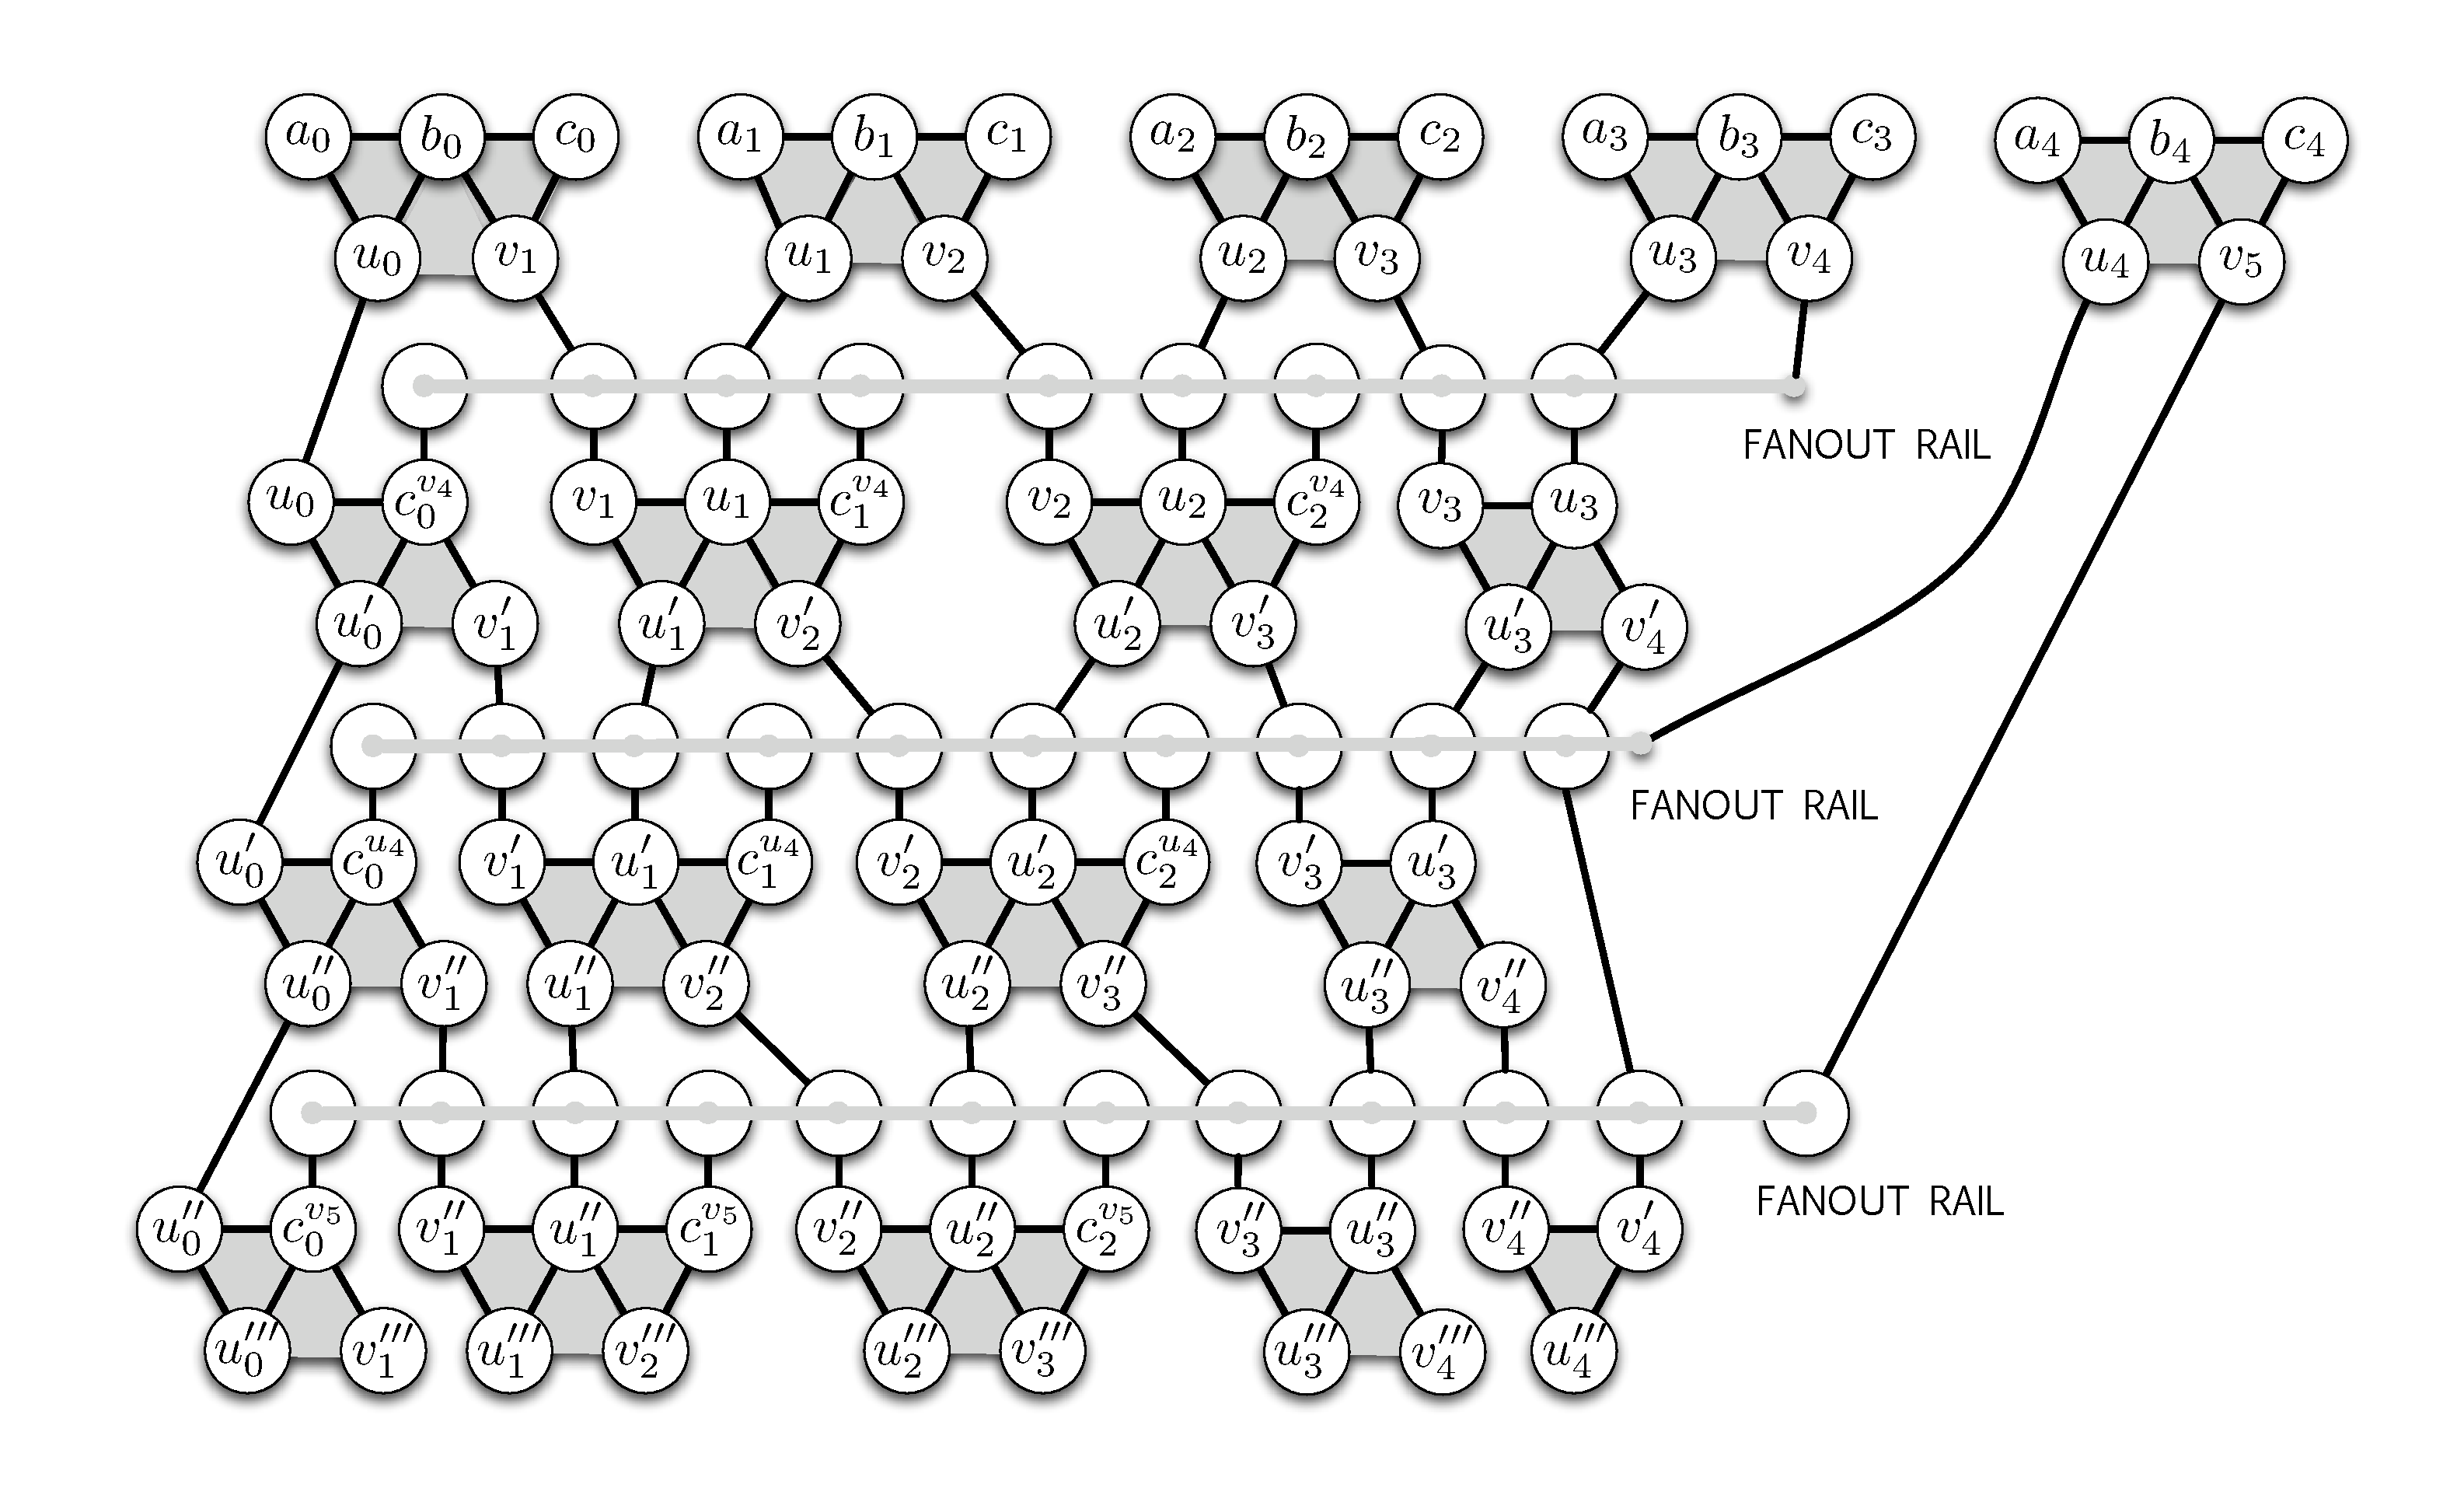
\includegraphics[width=6.5in]{factor-polylog/figures/mod-add-fixed.pdf}
}
\caption{Addition and three rounds of modular reduction for a 3-bit
modulus.}
\label{fig:csa-add-4}
\end{figure*}
\end{center}

A \textsc{2D CCNTC} circuit for modular addition of $5$-bit numbers using
four layers of parallel CSA's is shown graphically in Figure \ref{fig:csa-add-4}
which corresponds directly to the schematic proof in Figure \ref{fig:csa-proof}.
Note that in Figure \ref{fig:csa-add-4}, the least significant qubits are
on the left, and in Figure \ref{fig:csa-proof}, the least significant qubits are
on the right.
Figure \ref{fig:csa-add-4} also represents the approximate
physical layout of the qubits as they would look if this
circuit were to be fabricated.
Here, we convert the sum of three
$5$-bit integers into the modular sum of two $5$-bit integers, with a
$3$-bit modulus $m$.
In the first layer,
we perform 4 CSA's in parallel on the input numbers ($a,b,c$) and produce the
output numbers ($u, v$).

As described above, we truncate
the three high-order bits during the initial CSA round
(bits $u_4, v_4, v_5$) to retain a $4$-bit number.
Each of these bits serves as a control for adding its modular residue to
a running total. We can classically precompute $2^4[m]$ for the two
additions controlled on $u_4$ and $v_4$ and
$2^5[m]$ for the addition controlled on $v_5$.

In Layer 2,
we use a constant-depth fanout rail (see Figure \ref{fig:cdf}) to
distribute the control bit $v_4$ to its modular residue, which we denote as
%%\begin{equation}
$\ket{c^{v_4}} \equiv \ket{2^4[m]\cdot v_4}$.
%%\end{equation}
%This fanout requires constant depth;
The register $c^{v_4}$ has $n$ bits, which we add to the CSE results of layer 1.
The results $u_i$ and $v_{i+1}$ are teleported into layer 3. The exception is
$v'_4$ which is teleported into layer 4, since there are no other $4$-bits
to which it can be added. Wherever there are only
two bits of the same significance, we use the 2-2 adder from
Section \ref{sec:csa}.

Layer 3
%%, shown in Figure \ref{fig:csa-add-3},
operates similarly to layer 2, except that the modular residue is controlled on
$u_4$:
%%\begin{equation}
$\ket{c^{u_4}} \equiv \ket{2^4[m] \cdot u_4}$.
%%\end{equation}
%This fanout again requires constant depth;
The register $c^{u_4}$ has $3$ bits, which we
add to the CSE results of layer 2, where $u'_i$ and $v'_{i+1}$ are teleported
forward into layer 4.

Layer 4
%%, shown in Figure \ref{fig:csa-add-4},
is similar to layers 2 and 3, with the modular residue controlled on $v_5$:
%%\begin{equation}
$\ket{c^{v_5}} \equiv \ket{2^5[m] \cdot v_5}$.
%%\end{equation}
%This fanout is constant depth;
The register $c^{v_5}$ has $3$ bits, which we
add to the CSE results of layer 3.
There is no overflow bit $v'''_5$, and no carry bit from $v''_4$ and $v'_4$
as argued in the proof of Lemma 1.
The final modular sum $(a+b+c)[m]$ is $u'''+v'''$.

The general circuit for adding three $n$-qubit quantum integers to
two $n$-qubit quantum integers is called a \emph{CSA tile}. Each CSA tile in our architecture 
corresponds to its own module, and it will be represented by the symbol in 
Figure \ref{fig:csa-tile-symbol} for the rest of this paper. We call this
an $n$-bit modular adder, even though it accepts $(n+2)$-bit inputs, because
the size of the modulus is still $n$ bits.

\begin{center}
\begin{figure*}[h!bt]
\centerline{
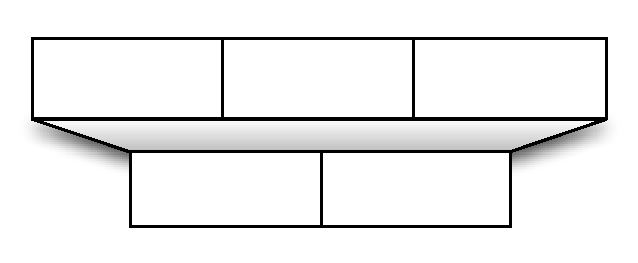
\includegraphics[width=1.5in]{factor-polylog/figures/csa-tile-symbol.pdf}
}
\caption{Symbol for an $n$-bit 3-to-2 modular adder, also called a CSA tile.}
\label{fig:csa-tile-symbol}
\end{figure*}
\end{center}


\subsection{Quantum Circuit Resources for Modular Addition}

We now calculate numerical upper bounds for the circuit resources of
the $n$-bit $3$-to-$2$ modular adder described in the previous section.
There are four layers of non-modular $n'$-bit $3$-to-$2$ adders, each of which
consists of $n'$ parallel single-bit adders whose
resources are detailed in Table \ref{tab:csa-tile-resources}. For factoring
an $n$-bit modulus, we have $n'=n+2$ in the first and fourth layers
and $n'=n+1$ in the second and third layers.

After each of the first three layers, we must move the output qubits
across the fanout rail to be the inputs of the next layer. We use
two swap gates, which have a depth and size of $6$ CNOTs each, since
the depth of teleportation is only more efficient for moving more than
two qubits. The control bit for each modular residue needs to be
teleported $0$, $4$, and $7$ qubits respectively according to the
diagram in Figure \ref{fig:csa-add-4}, before being fanned out $n$
times along the fanout rails, where the fanned out copies will end up
in the correct position to be added as inputs.

%The detailed resources for a Toffoli gate and the single-bit adder that uses
%them are given in Table \ref{tab:csa-tile-resources}.

The resources for the $n$-bit $3$-to-$2$ modular adder depicted in Figure
\ref{fig:csa-add-4} are given below.
The formulae reflect the resources needed for both computing the output
in the forward direction (including creating an entangled fanned-out state
controlled on overflow qubits)
and also uncomputing ancillae in the backward
direction (including disentangling previous fanned-out copies).

The circuit depth is $O(1)$:

\begin{equation}
374\text{.}
\end{equation}

The circuit size is $O(n)$:

\begin{equation}
551n + 757\text{.}
\end{equation}

The circuit width is $O(n)$:

\begin{equation}
33n + 47\text{.}
\end{equation}

\section{Quantum Modular Multiplication}
\label{sec:csa-mod-mult}

We can build upon our carry-save adder to implement quantum modular
multiplication in logarithmic depth. We start with a completely classical
problem to illustrate the principle of multiplication by repeated addition.
Then we consider modular multiplication of two quantum integers in a serial
and a parallel fashion in Section
\ref{subsec:csa-mod-mult-qq}. Both of these problems use as subroutines
\emph{partial product creation}, which we define and solve
 in Section \ref{subsec:ppc} and
 \emph{modular multiple addition}, which we define and solve
in Section \ref{subsec:mma}.

%%%%%%%%%%%%%%%%%%%%%%%%%%%%%%%%%%%%%%%%%%%%%%%%%%%%%%%%%%%%%%%%%%%%%%%%%%%%%%%
First we consider a completely classical problem:
given three $n$-bit classical numbers $a$, $b$, and $m$,
compute $c = ab \bmod m$, where $c$ is allowed to be in CSE.

We only have to add shifted
multiples of $a$ to itself, ``controlled'' on the bits of $b$. There are
$n$ shifted multiples of $a$, let's call them $z^{(i)}$, one for every bit of $b$:
%%\begin{equation}
$z^{(i)} = 2^i a b_i \bmod m$.
%%\end{equation}
We can parallelize the addition of $n$ numbers in a logarithmic depth
binary tree to get a total depth of $O(\log n)$.

%%%%%%%%%%%%%%%%%%%%%%%%%%%%%%%%%%%%%%%%%%%%%%%%%%%%%%%%%%%%%%%%%%%%%%%%%%%%%%
\subsection{Modular Multiplication of Two Quantum Integers}
\label{subsec:csa-mod-mult-qq}

We now consider the problem of multiplying a classical number controlled
on a quantum bit with a
\emph{quantum integer}\footnote{In this paper, an $n$-qubit 
quantum integer is a
general superposition of up to $2^n$ classical integers. As a special case,
a classical number controlled on a single qubit is a superposition of
$2$ classical integers.},
which is a
quantum superposition of classical numbers:

\begin{quote}
Given an $n$-qubit quantum integer $\ket{x}$, a control qubit $\ket{p}$,
and two $n$-bit classical numbers $a$
and $m$,
compute $\ket{c} = \ket{xa[m]}$, where $c$ is allowed to be in CSE.
\end{quote}

This problem occurs naturally in modular exponentiation (described in
the next section) and can be considered \emph{serial multiplication},
in that $t$ quantum integers are multiplied in series to a single
quantum register. This is used in serial QPF as mentioned in
Section \ref{sec:related}.


We first create $n$ quantum integers $\ket{z^{(i)}}$,
which are shifted multiples of the classical number $a$ controlled on the bits
of $x$:
%\begin{equation}
$\ket{z^{(i)}} \equiv \ket{2^i a[m] \cdot x_i }$.
%\end{equation}
These are typically called \emph{partial products} in a classical multiplier.
How do we create these numbers, and what is the depth of the procedure?
First, note that $\ket{2^i a[m]}$ is a classical number, so we can
precompute them classically and prepare them in parallel using single-qubit
operations
on $n$ registers, each consisting of $n$ ancillae qubits. Each $n$-qubit
register will hold a future $\ket{z^{(i)}}$ value.
We then fan out each of the
$n$ bits of $x$, $n$ times each, using an unbounded fanout operation so that
$n$ copies of each bit $\ket{x_i}$ are next to register $\ket{z^{(i)}}$.
This takes a total of $O(n^2)$ parallel CNOT operations.
We then entangle each $\ket{z^{(i)}}$ with the corresponding $x_i$.
%The schematic for this is shown in Figure \ref{fig:mod-mult-create}.
After this, we interleave these numbers into groups of three using
constant-depth teleportation. This reduces to the task of modular
multiple addition in order to add these numbers down to a single
(CSE) number modulo $m$, which is described in Section \ref{subsec:mma}.

%\begin{figure*}[htp!]
%\centerline{
%\includegraphics[width=4.5in]{./znumbers.pdf}
%}
%\caption{Creating $n=4$ shifted values $\{z^{(0)},z^{(1)},z^{(2)},z^{(3)}\}$
%for an input number $x$.}
%\label{fig:mod-mult-create}
%\end{figure*}

Finally, we tackle the most interesting problem:
\begin{quote}
Given two $n$-qubit quantum integers $\ket{x}$ and
$\ket{y}$ and an $n$-bit classical number
$m$,
compute $\ket{c} = \ket{xy \bmod m}$,
where $\ket{c}$ is allowed to be in CSE.
\end{quote}

This can be considered \emph{parallel multiplication} and is responsible
for our logarithmic speedup in modular exponentiation and parallel QPF.


Instead of creating $n$ quantum integers $\ket{z^{(i)}}$, we must create
up to $n^2$ numbers
$\ket{z^{i,j}}$ for all possible pairs of quantum bits $x_i$ and $y_j$,
$i,j \in \{0,\ldots,n-1\}$:
%\begin{equation}
$\ket{z^{i,j}} \equiv \ket{2^i2^j[m]\cdot x_i \cdot y_j}$.
%\end{equation}
We create these numbers using a similar procedure to the previous problem.
Adding $n^2$ quantum integers of $n$ qubits each takes depth
$O(\log(n^2))$, which is still $O(\log n)$.
Creating $n^2\times n$-bit quantum integers takes width $O(n^3)$.
Numerical constants are given for these resource estimates in
Section \ref{subsec:mod-mult-resources} for the entire modular multiplier.

Here is an outline of our modular multiplier construction, combining the
two halves of partial product creation (Section \ref{subsec:ppc}) and
modular multiple addition (Section \ref{subsec:mma}).

\begin{enumerate}
\item Initially, the inputs consist of the CSE quantum integers $x$ and $y$,
each with $2n+3$ bits, sitting on adjacent edges of a square lattice that has
sides of length $3(2n+3)$ qubits.
\item For each of $\lceil \log_2 (2n+3) \rceil$ rounds:
\begin{enumerate}
\item Of the existing $\{x_i\}$ and $\{y_j\}$ bits, apply a CNOT to create an
entangled copy in an adjacent qubit.
\item Teleport this new copy halfway between its current location and the
new copy.
\item At every site where an $\ket{x_i}$ and an $\ket{y_j}$ meet,
apply a Toffoli gate to create $\ket{x_i \cdot y_j}$.
\item Teleport $\ket{x_i \cdot y_j}$ to the correct $z$-site module.
\end{enumerate}
\item Within each $z$-site module, fanout $\ket{x_i \cdot y_j}$ up to $n$
times, corresponding to each $1$ in the modular residue $2^i 2^j \bmod m$,
to create the $n$-qubit quantum integer $\ket{z^{(i,j)}}$.
\item For each triplet of $z$-site modules, teleport the quantum integers
$\ket{z^{(i,j)}}$ to a CSA tile module, interleaving the three numbers so that
bits of the same significance are adjacent. This concludes partial product
creation (Section \ref{subsec:ppc}).
\item Perform modular multiple addition (described in Section \ref{subsec:mma})
on $t'$ $n$-qubit quantum integers down to 2 $n$-qubit quantum integers (one CSE number).
\item Uncompute all the previous steps to restore ancillae to $\ket{0}$.
\end{enumerate}
%%%%%%%%%%%%%%%%%%%%%%%%%%%%%%%%%%%%%%%%%%%%%%%%%%%%%%%%%%%%%%%%%%%%%%%%%%%%%%%
\subsection{Partial Product Creation}
\label{subsec:ppc}

This subroutine describes the procedure of creating $t'=O(n^2)$ partial products of
the CSE quantum integers $x$ and $y$, each with $2n+3$ bits each. We will now
discuss only the case of parallel multiplication. Although we
will not provide an explicit circuit for this subroutine, we will outline
our particular construction and give a numerical upper bound on the
resources required.

First, we need to generate the product bits
$\ket{x_i\cdot y_j}$ for all possible $(2n+3)^2$ pairs of $\ket{x_i}$ and
$\ket{y_j}$.
A particular product bit $\ket{x_i \cdot y_j}$
controls a particular classical number, the
$n$-bit modular residue $2^i 2^j [m]$, to form the partial product
$\ket{z^{(i,j)}}$ defined
in the previous section. However, some of these partial products
consist of only a single qubit, if $2^i 2^j < 2^n$, which is the minimum
value for an $n$-bit modulus $m$. There are at least $2n^2 - 2n + 1$
such single-bit partial products, which can be grouped into at most
$(2n+3)\times n$-bit numbers. Of the $(2n+3)^2$ possible partial products,
this leaves the number of remaining $n$-bit partial products as at most
$2n^2 + 14n +8$. Therefore we have a maximum number of $n$-bit
partial products, which we will simply refer to as $t'$ from now on.

\begin{equation}
t'=2n^2+16n+11
\label{eqn:tprime}
\end{equation}

The creation of the product bits $\ket{x_i \cdot y_j}$ occurs on a
square lattice of $(3(2n+3))^2$ qubits, with the numbers $\ket{x_i}$ and
$\ket{y_j}$ located on adjacent edges. The factor of $3$ in the size of the lattice
allows the $\ket{x_i}$ and $\ket{y_j}$ bits move past each other.
The $\ket{x_i}$ bits are teleported along an axis that is perpendicular to
the teleportation axis for the $\ket{y_j}$ bits, and vice versa.
Product bit creation, and this square lattice, comprise a single module.
In $\lceil \log_2 (2n+3) \rceil$
rounds, these bits are copied via a CNOT and teleported to the middle of
a recursively halved interval of the grid. The copied bits $\ket{x_i}$ and
$\ket{y_j}$
first form $1$ line, then $3$ lines, then $7$ lines, and so forth,
intersecting at $1$ site, then $9$ sites, then $49$ sites, and so forth.
There are $\lceil \log_2 (2n+3) \rceil$ such rounds.

At each intersection, a Toffoli gate is used to create $\ket{x_i \cdot y_j}$
from the given $\ket{x_i}$ and $\ket{y_j}$. These product bits are then
teleported away from this qubit, out of this product bit module, to different
modules where the $\ket{z^{(i,j)}}$ numbers are later generated,
called $z$-sites. There are $t'$ $z$-site modules which each contain 
an $n$-qubit quantum integer. Any
round of partial product generation will produce at most as many product
bits $x_i \cdot y_j$ as in the last round, which is half the total number
of $(2n+3)^2$.
%These product bits are teleported out the two sides of the
%square lattice that are opposite the input numbers $x$ and $y$, which means the
%square lattice has dimension at most $((2(2n+3)-1)(n+2))^2 = O(n^4)$.

%The $z$-sites have total width of $3nt'$ qubits, so the maximum total
%teleportation length of all qubits is $(2n+3)^2$ multiplied by the maximum
%length of any single teleportation length,
%Our construction consists of the following steps:

We now present the resources for partial product creation, the first half of
a modular multiplier, including the reverse computation.

The circuit depth is $O(\log n)$:

\begin{equation}
D_{PPC} = 32\log_2 n + 150\text{.}
\end{equation}

The module depth is $O(1)$:

\begin{equation}
\overline{D}_{PPC} = 8\text{.}
\end{equation}

The circuit size is $O(n\log^2 n)$:

\begin{eqnarray}
S_{PPC} & = & (6n + 9)\log_2 n +\\
        &   & (26n^3 + 232n^2 + 224n + 159)\text{.}
\end{eqnarray}

The module size is $O(n^2)$:

\begin{eqnarray}
\overline{S}_{PPC} = 6n^2 + 26n + 19\text{.}
\end{eqnarray}

The circuit width is $O(n^3)$:

\begin{eqnarray}
W_{PPC} = 6n^3 + 48n^2 - 8n + 1\text{.}
\end{eqnarray}

The module width is $O(n^2)$:

\begin{eqnarray}
\overline{W}_{PPC} = 2n^2 + 14n + 9\text{.}
\end{eqnarray}

%%%%%%%%%%%%%%%%%%%%%%%%%%%%%%%%%%%%%%%%%%%%%%%%%%%%%%%%%%%%%%%%%%%%%%%%%%%%%%%
\subsection{Modular Multiple Addition}
\label{subsec:mma}

As a subroutine to modular multiplication, we define the operation of
repeatedly adding multiple numbers down to a single CSE number, called
\emph{modular multiple addition}.

The modular multiple addition circuit generically adds down $t'\times n$-bit
conventional numbers to an $n$-bit CSE number:
%
\begin{equation}
z^{(1)} + z^{(2)} + \ldots z^{(t')} \equiv (u+v)[m].
\end{equation}
%
It does not matter how the
$t'$ numbers are generated, as long as they are divided into groups of three
and have their bits interleaved to be the inputs of a CSA tile.
From the previous section, serial multiplication results in
$t' \le n$ and parallel multiplication results in $t' \le n^2$. Each CSA tile
is contained in its own module. These modules are arranged in layers within
a logarithmic depth binary tree, where 
the first layer contains $\lceil t'/3 \rceil$ modules. A modular addition
occurs in all the modules of the first layer in parallel. The outputs from this
first layer are then teleported to be the inputs of the next layer of modules,
which have at most two-thirds as many modules. This continues until the
tree terminates in a single module, whose output is a CSE number $u+v$ which
represents the modular product of all the original $t'$ numbers. The resulting
height of the tree is $(\lceil \log_{3/2}(t'/3) \rceil + 1)$ modules.

As the parallel modular additions proceed by layers, all previous layers
must be maintained in a coherent state, since the modular addition leaves
garbage bits behind. Only at the end of modular multiple addition, after
the final answer $u+v$ is obtained, can all the previous layers be
uncomputed in reverse to free up their ancillae.

These steps are best illustrated with a concrete
example in Figure \ref{fig:mod-mult}. The module for each CSA tile is
represented by the symbol from Figure \ref{fig:csa-tile-symbol}.
The arrows indicate the
teleportation of output numbers from the source tile to be input numbers
into a destination tile.

\begin{figure*}[htb!]
\centerline{
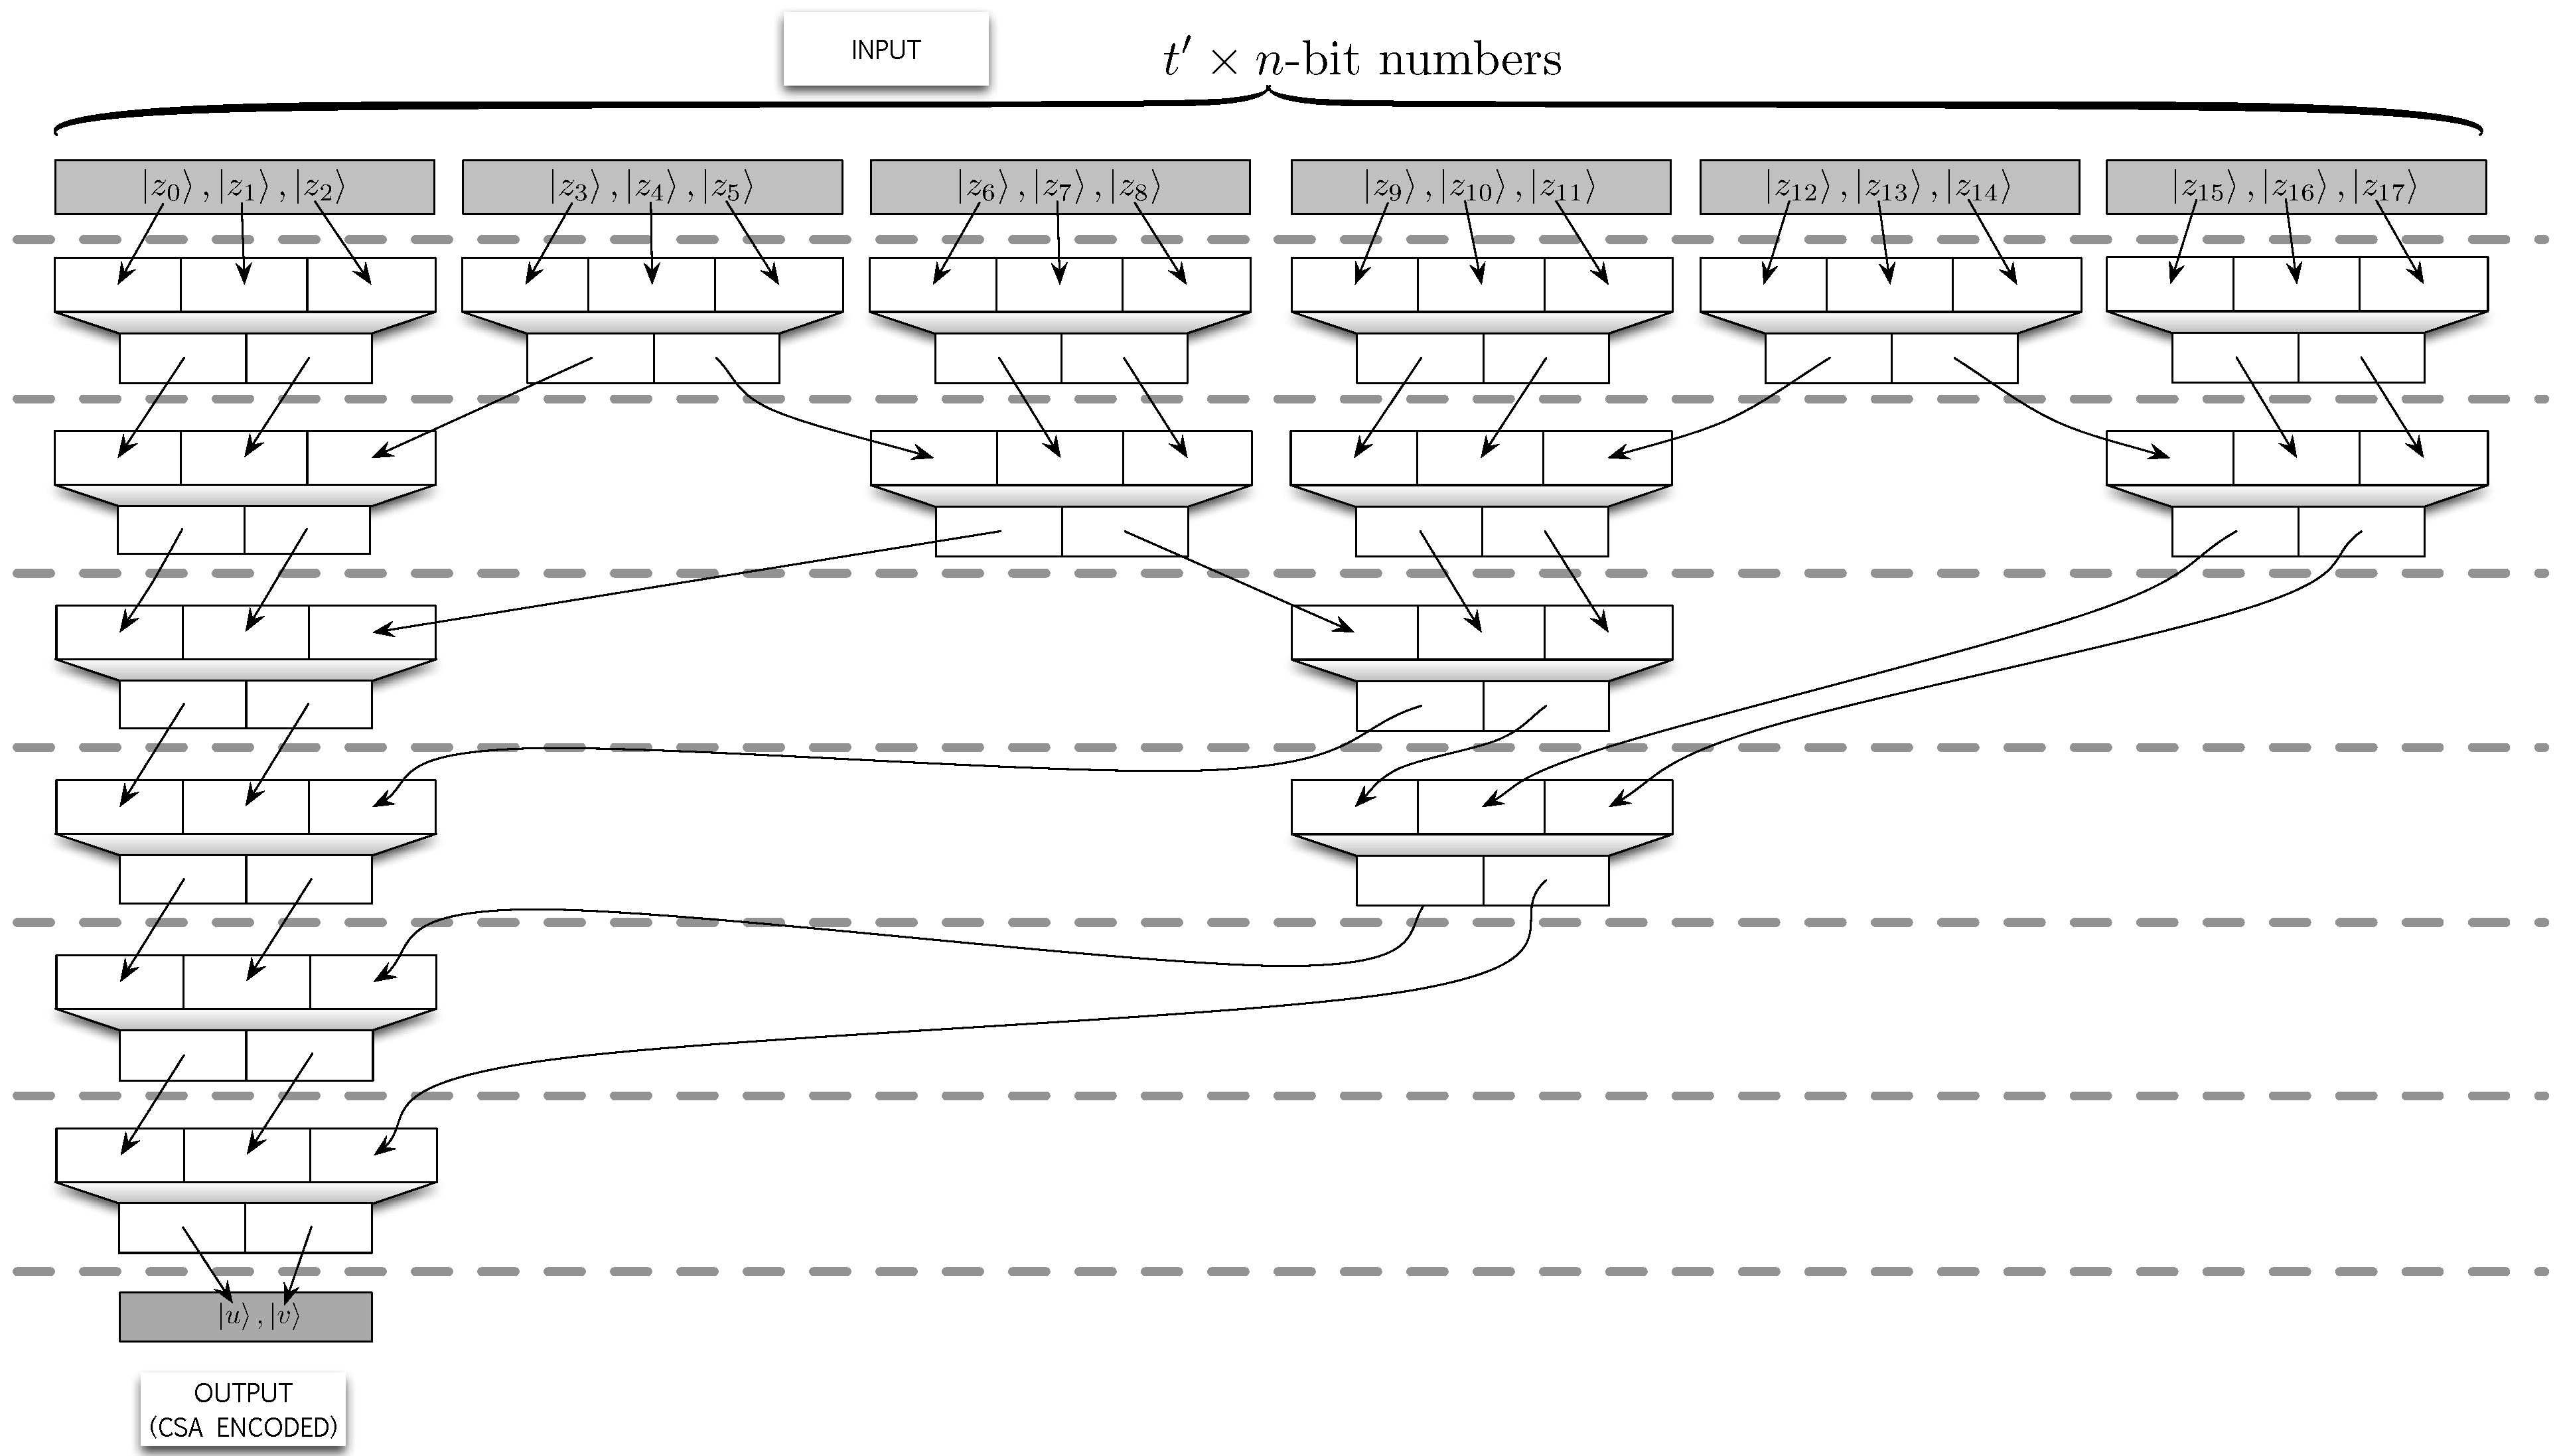
\includegraphics[width=5.5in]{factor-polylog/figures/mod-mult-add.pdf}
}
\caption{Modular multiple addition of quantum integers on a CSA tile
architecture for $t'=18$ in a logarithmic-depth tree with height $(\lceil \log_{\frac{3}{2}}(t'/3) \rceil + 1) = 6$. Arrows represent teleportation
in between modules.}
\label{fig:mod-mult}
\end{figure*}
%

Now we can analyze the circuit resources for multiplying $n$-bit
quantum integers, which requires $(t'-2)$ modular additions, for $t'$ from
Equation \ref{eqn:tprime}.
The circuit width is the sum of the $O(n^3)$ ancillae
needed for partial product creation and the ancillae required for $O(n^2)$
modular additions. Each modular addition has width $O(n)$ and depth $O(1)$
from the previous
section. There are
$\lceil \log_{3/2}(n^2 / 3) \rceil +1 $ timesteps of modular addition. Therefore
the entire modular multiplier circuit has depth $O(\log n)$ and width $O(n^3)$.

\subsection{Modular Multiplier Resources}
\label{subsec:mod-mult-resources}.

The circuit depth of the entire modular multiplier is $O(\log n)$:

\begin{equation}
D_{MM} = 1383 \log_2 n + 3930\text{.}
\end{equation}

The module depth is $O(\log n)$:
\begin{equation}
\overline{D}_{MM} = 2\log_2 n + 11\text{.}
\end{equation}

The circuit size is $O(n^3)$:

\begin{eqnarray}
S_{MM} = & (6n + 9)\log_2 n +\\
        & (1152n^3 + 10780n^2 + 17628n + 7082)\text{.}
\end{eqnarray}

The module size is $O(n^3)$:

\begin{equation}
\overline{S}_{MM} = 15n^3 + 127n^2 + 178n + 50{.}
\end{equation}

The circuit width is $O(n^3)$:

\begin{equation}
W_{MM} = 66n^3 + 558n^2 + 870n + 290\text{.}
\end{equation}

The module width is $O(n^2)$:

\begin{equation}
\overline{W}_{MM} = 4n^2 + 28n + 15\text{.}
\end{equation}

\section{Quantum Modular Exponentiation}
\label{sec:modexp}

We now extend our arithmetic to modular exponentiation, which is repeated
modular multiplication controlled on qubits supplied by a phase estimation
procedure.
If we wish to multiply an $n$-qubit quantum input number $\ket{x}$ by
$t$ classical numbers $a^{(j)}$, we can multiply them in series.
% as shown in
%Figure \ref{fig:modexp-qc-series}.
This requires depth $O(t\log n)$ in modular multiplication operations.

%\begin{figure}[htp!]
%\begin{center}
%\includegraphics[width=5.5in]{figures/modexp-qc-series.pdf}
%\end{center}
%\caption{Multiplying a quantum number $\ket{x}$ by $t$ classical numbers
%$\{a^{0}, a^{1}, \ldots, a^{n-1}\}$ in series.}
%\label{fig:modexp-qc-series}
%\end{figure}

Now consider the same procedure, but this time each classical number $a^{(j)}$
is controlled on a quantum bit $p_j$. This is a special case of
multiplying by $t$ quantum integers in series, since a classical number
entangled with a quantum integer is also quantum.
%This is shown in
%Figure \ref{fig:modexp-qq-series}.
It takes the same depth $O(t\log n)$ as the previous case.
%
%\begin{figure}[htp!]
%\begin{center}
%\includegraphics[width=5.5in]{figures/modexp-qq-series.pdf}
%\end{center}
%\caption{Multiplying a quantum number $\ket{x}$ by $t$ quantum numbers
%$\{\ket{a^{0}p_0}, \ket{a^{1}p_1}, \ldots, \ket{a^{n-1}p_{n-1}}\}$ in series.}
%\label{fig:modexp-qq-series}
%\end{figure}

Finally, we consider multiplying $t$ quantum integers
$\{x^{(1)}, x^{(2)}, \ldots, x^{(t-1)}, x^{(t)}\}$ in a parallel,
logarithmic-depth binary tree.
This is shown in Figure \ref{fig:modexp-qq-parallel}, where arrows indicate multiplication.
The tree has depth $\log_2(t)$ in modular multiplier operations. Furthermore,
each
modular multiplier has depth $O(\log(n))$ and width $O(n^3)$ for $n$-qubit
numbers. Therefore, the overall depth of this parallel modular exponentiation
structure is $O(\log(t)\log(n))$ with width $O(tn^3)$.
In phase estimation for QPF, it is
sufficient to take $t = O(n)$ \cite{Nielsen2000,Kitaev2002}. Therefore our total depth is
$O(\log^2(n))$ and our total size and total width are $O(n^4)$, as desired. At this point, combined with the parallel phase
estimation procedure of \cite{Kitaev2002}, we have a complete factoring
implementation in our hybrid 2D nearest-neighbor architecture in poly-logarithmic
depth.
%
\begin{figure*}[tb!]
\centerline{
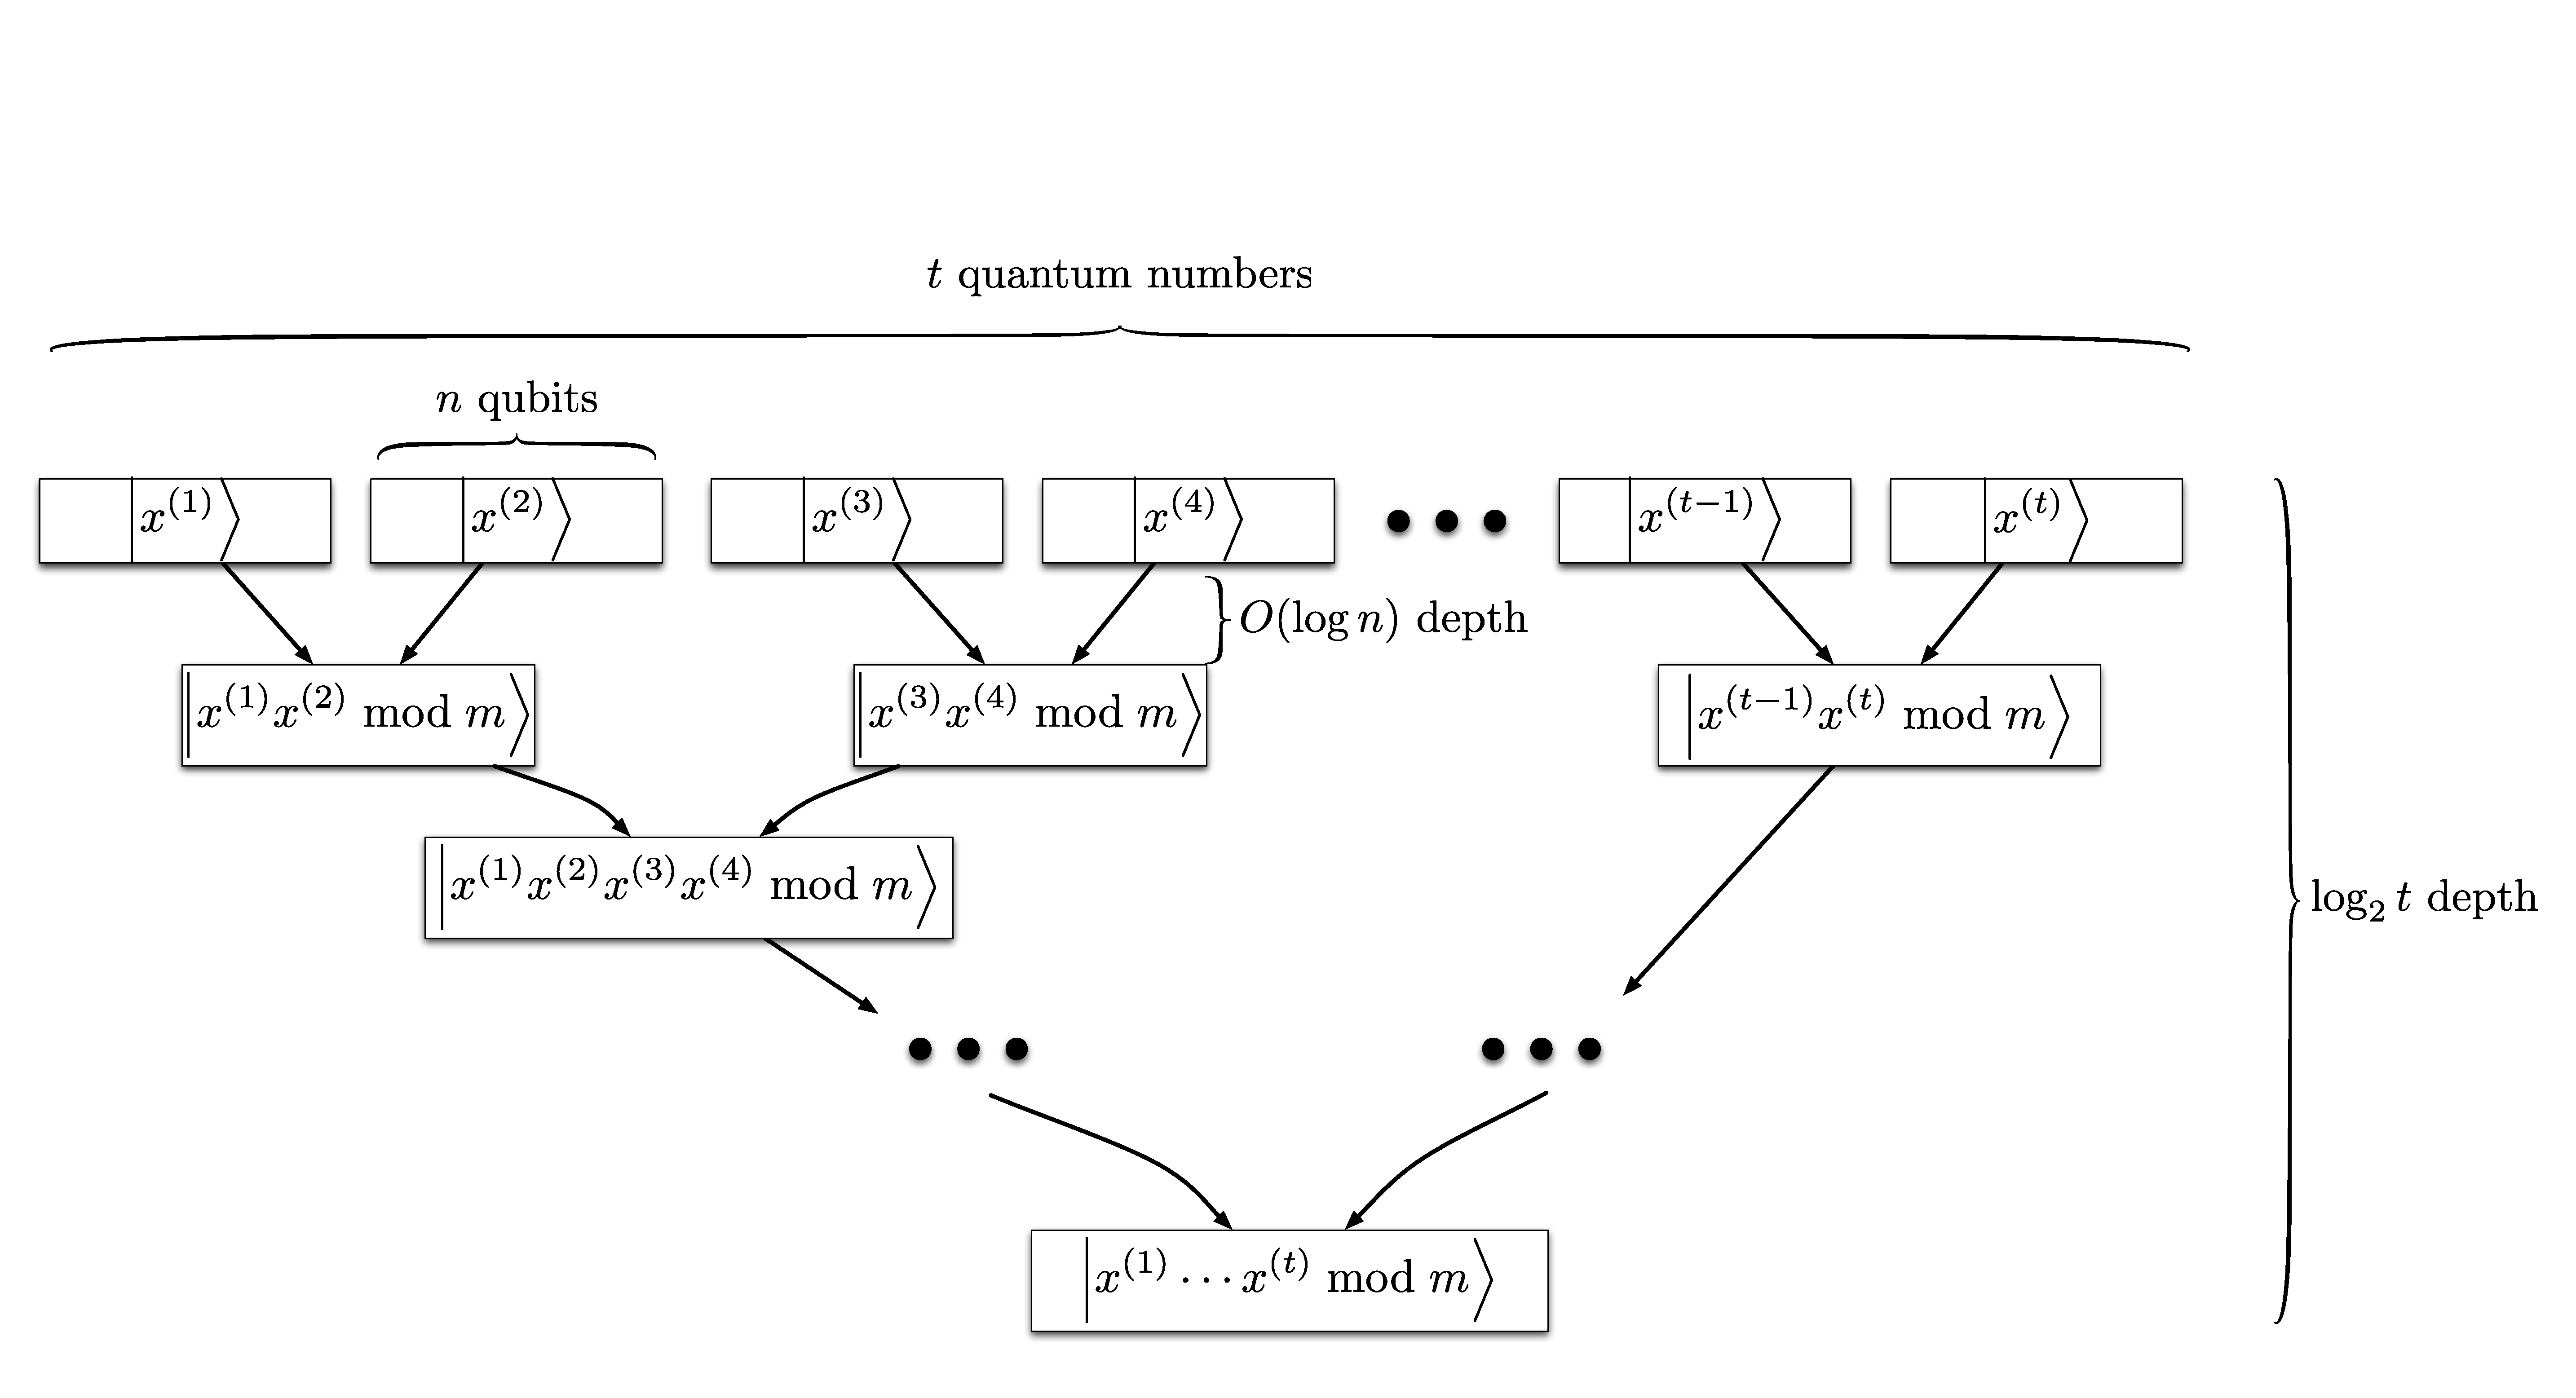
\includegraphics[width=5.5in]{factor-polylog/figures/mod-exp-par.pdf}
}
\caption[Parallel modular exponentiation]
{Parallel modular exponentiation: multiplying $t$ quantum integers
%$\{\ket{x^{(0)}}, \ket{x^{(1)}}, \ldots, \ket{x^{(t-1)}}\}$ in parallel,
in a $O(\log{(t)}\log{(n)})$-depth binary tree. Arrows indicate modular
multiplication.}
\label{fig:modexp-qq-parallel}
\end{figure*}

We will now calculate numerical
constants to upper bound circuit resources.

According to the Kitaev-Shen-Vyalyi parallelized phase estimation procedure
\cite{Kitaev2002},
for a constant success probability of $3/4$,
it is sufficient to multiply together $t = 2867n$ quantum integers,
controlled on the qubits $\ket{p_j}$, in parallel.

In Section \ref{subsec:qcla}, we describe the last step of modular
exponentiation in CSE. In Section \ref{subsec:modexp-resources}, we
state the final circuit resources for the entire modular exponentiation
circuit,
and therefore, our quantum period-finding procedure.

%%%%%%%%%%%%%%%%%%%%%%%%%%%%%%%%%%%%%%%%%%%%%%%%%%%%%%%%%%%%%%%%%%%%%%%%%%%%%%
\subsection{Converting Back to a Unique Conventional Number}
\label{subsec:qcla}

The final product of all $t$ quantum integers is in CSE which is not
unique. As stated in Gossett's original paper \cite{Gossett1998}, this
must be converted back to a conventional number using, for example, the
quantum carry-lookahead adder (QCLA) from \cite{Draper2004}. We can convert
this to a nearest-neighbor architecture by using the qubit reordering
construction of \cite{Rosenbaum2012}. We now compute the resources
needed for this last step.

To add two $(n+2)$-bit numbers in a QCLA, we have a circuit width of
$k = (4(n+2) - 2\log_2 n - 1)$. The depth is at most $4\log_2 n +2$ gates,
and some of them act on qubits that are not nearest-neighbors. Therefore,
we add in between each gate a reordering circuit that takes $k^2$
(reusable) ancillae
qubits and uses two rounds of constant-depth teleportation to rearrange
the qubits into a new order where all the gates are nearest-neighbor.
Adding in the teleportation circuit resources from Table \ref{tab:cd-resources},
we can calculate the following resources.

The circuit depth is $O(\log n)$:
%
\begin{equation}
D_{QCLA} = 56\log_2 n + 28\text{.}
\end{equation}
%
The circuit size is $O(n^2 \log n)$:
%
\begin{eqnarray}
S_{QCLA} = 96 \log_2^3 n & - & (384n + 624)\log_2^2 n \nonumber \\
              & + & (384n^2 + 1152n + 840) \log_2 n \nonumber \\
              & + & (192n^2 + 672n + 588)\text{.}
\end{eqnarray}
%
The circuit width is $O(n^2)$:
%
\begin{equation}
W_{QCLA} = 4 \log_2^2 n - (16n + 30)\log_2 n + 16n^2 + 60n + 56\text{.}
\end{equation}


%%%%%%%%%%%%%%%%%%%%%%%%%%%%%%%%%%%%%%%%%%%%%%%%%%%%%%%%%%%%%%%%%%%%%%%%%%%%%%
\subsection{Circuit Resources for Modular Exponentiator}
\label{subsec:modexp-resources}

This leads to the following circuit resource upper bounds for a modular exponentiator. Therefore, these are the total resources for running a
single round of parallel QPF as part of Shor's factoring algorithm.

The circuit depth is $O(\log^2 n)$:
% From Notebook #16 p. 225, N18, p. 3-4
\begin{equation}
D_{ME} = 1383\log_2^2(n) + 21253\log_2(n) + 49098\text{.}
\end{equation}
%
The module depth is $O(\log^2 n)$:
%
\begin{equation}
\overline{D}_{ME} = 3\log_2 n + 24
\end{equation}
%
The circuit size is $O(n^4)$:
%
\begin{eqnarray}
S_{ME} & = & 96 \log_2^3 n + \nonumber \\
       & - & (384n + 624)\log_2^2 n \nonumber \\
       & + & (384n^2 + 1152n + 840) \log_2 n \nonumber \\
       &   & 3302324 n^4 + 30900797 n^3 + 50527571 n^2  + 20287173 n + 
  -6494\text{.}
\label{eqn:sme}
\end{eqnarray}
%
The module size is $O(n^4)$:
%
\begin{eqnarray}
\overline{S}_{ME} & = & (17202 n^2 + 25797 n - 9) \log_2 n + \nonumber \\
                  & + & 3302784 n^4 + 30905108 n^3 50534430 n^2 + 20295063 n - 7088 \text{.}
\end{eqnarray}
%
The circuit width is $O(n^4)$:
%
\begin{equation}
W_{ME} = 94598n^4 + 799749 n^3 + 1246692 n^2 + 418089 n - 145\text{.}
\end{equation}
%
The module width is $O(n^3)$:
%
\begin{equation}
\overline{W}_{ME} = 5736 n^3 + 40152 n ^2 + 21510 n\text{.}
\end{equation}

\section{Asymptotic Results}
\label{sec:fpl-results}

The asymptotic resources required for our approach,
as well as the resources for other nearest-neighbor approaches,
are listed in Table \ref{tab:fpl-results},
where we assume a fixed constant error
probability for each round of QPF. Not all resources are
provided directly by the referenced source.

Resources in square brackets
are inferred using Equation \ref{eqn:depth-width}.
These upper bounds are correct,
but may not be tight with the upper bounds
calculated by their respective authors.
In particular, a more detailed analysis
could give a better upper bound for circuit size than the
depth-width product. Also note that the
work by Beckman et al. \cite{Beckman1996} is unique in that it uses
efficient multi-qubit gates inherent to linear ion trap technology which at first
seem to
be more powerful than \textsc{1D NTC}. However, use of these gates does not result in an
asymptotic improvement over \textsc{1D NTC}.

%, say $\epsilon=1/4$.
% and $\delta' = 1/2$ for KSV-QPF.
%Note that the
%number of measurements are included for completeness.
%, since these are
%not counted as gates in our model but may be comparable in terms of
%execution time.
%Some table cells are blank if the entries are not relevant to the current comparison, or if the entires were not %calculated in the prior work.
We achieve an exponential
improvement in nearest-neighbor circuit depth (from quadratic to polylogarithmic)
with our approach at the cost of a polynomial increase in
circuit size and width. Similar depth improvements at the cost of width increases can be achieved using the modular multipliers
of other factoring implementations
by arranging them in a parallel modular exponentiator.
Our approach is the first implementation for factoring on \textsc{2D NTC},
augmented with a classical controller and parallel, communicating
modules (\textsc{\textsf{2D CCNTCM}}).
%
\begin{table}[htb!]
\begin{center}
\begin{tabular}{|c|c|c|c|c|}
\hline
Implementation             & Architecture      & Depth   & Size   & Width     \\
\hline
Vedral, et al. \cite{Vedral1996}   & \textsc{AC}      & $[O(n^3)]$ & $O(n^3)$    & $O(n)$ \\
Gossett \cite{Gossett1998}                   & \textsc{AC}       & $O(n \log n)$  & $[O(n^3\log n)]$  & $O(n^2)$  \\
Beauregard \cite{Beauregard2002}                & \textsc{AC}       & $O(n^3)$      & $O(n^3 \log n)$ & $O(n)$ \\
Zalka \cite{Zalka1998}                     & \textsc{AC}       & $O(n^2)$      & $[O(n^3)]$ & $O(n)$     \\
Takahashi \& Kunihiro \cite{Takahashi2006}     & \textsc{AC}       & $O(n^3)$      & $O(n^3\log n)$ & $O(n)$ \\
Cleve \& Watrous \cite{Cleve2000}           & \textsc{AC}       & $O(\log^3 n)$ & $O(n^3)$ & $[O(n^3 / \log^3n)]$ \\
\hline
Beckman et al. \cite{Beckman1996} & \textsc{Ion trap}   & $O(n^3)$ & $O(n^3)$ & $O(n)$\\
\hline
Fowler, et al. \cite{Fowler2004} & \textsc{1D NTC}   & $O(n^3)$ & $O(n^4)$ & $O(n)$\\
Van Meter \& Itoh \cite{VanMeter2006} & \textsc{1D NTC}   & $O(n^2 \log n)$ & $[O(n^4\log n)]$ & $O(n^2)$\\
Kutin \cite{Kutin2006}                     & \textsc{1D NTC}   & $O(n^2)$ & $O(n^3)$ & $O(n)$\\
\hline
Current Work               & \textsc{\textsf{2D CCNTCM}}   & $O(\log^2{n})$ & $O(n^4)$ & $O(n^4)$   \\
\hline
\end{tabular}
\end{center}
\caption{Asymptotic circuit resource usage for quantum factoring of an $n$-bit number.}
\label{tab:fpl-results}
\end{table}

\section{Conclusion}
\label{sec:fpl-conclude}

In this chapter, we've presented the first main result of
our dissertation in Section \ref{sec:mod-exp}:
factoring on a hybrid nearest-neighbor architecture in polylogarithmic depth.
We've place it in the context of previous factoring implementations on a
variety of different models. We provided a firm grounding
in the carry-save technique before using it to construct
a modular adder, a modular multiplier, and finally a
modular exponentiator. Combining the carry-save technique
with constant-depth
communication and parallel phase estimation yielded
this exponential improvement over the previous
state-of-the-art, a quadratic-depth nearest-neighbor
factoring architecture.

We have also examined the
effect of introducing modules by comparing our
implementation on both a hybrid model \textsf{2D CCNTCM}
and a non-hybrid model \textsf{2D CCNTC}.
Our hybrid model has reduced circuit resources
($D$, $S$, $W$) which better
capture the essential computational locality of Shor's factoring
algorithm while measuring part of the communication
costs in the module resources ($\overline{D}$, $\overline{S}$, $\overline{W}$).

The key point in this chapter is that
low-depth (sub-linear) factoring is possible
on a hybrid nearest-neighbor architecture
at only a polynomial increase in circuit size
and 
circuit width. It is possible to decrease
circuit size and width further by increasing
module size and module width.

Using our numerical
upper bounds, we can compute the amount of
physical resources to compromise a $4096$-bit
RSA key, currently regarded as a secure key size
for at least several decades. At a rate of
1 millisecond per timestep or long-range
teleportation, our implementation would
complete in 10 days.
 Our architecture
would require 5,736 communicating quantum
computers. If each quantum computer generated
enough entangled pairs for long-range
teleportation at a rate of 1 Hz, it would
take 4.5 hours to generate all required pairs.
At the current cost of residential electricity 
in Seattle of 10.71 cents per kilowatt-hour,
the architecture would cost $2.8$ billion
to power.
 Given a typical
separation of ions of 5 microns\footnote{Provided by Tom Noel for barium ions in the lab of Boris Blinov.},
the entire apparatus would occupy at least 1.26
square miles, about twice the land area of the city
of Seattle. Such figures, while large, are
within the realm of possibility in 50 years, especially
for governments.\footnote{For example,
1.26 square miles in low earth orbit would be cheap.
However, the commute would be quite expensive.}

Even if our figures were off by an order of magnitude,
our results would still confirm our thesis. We
would have provided a quantum architecture to solve
the human problem of factoring that is
buildable and runnable within the author's lifetime.
However, progress rarely stops with what is
feasible and usually moves on to what is possible.
Can the depth of factoring be improved even futher?
This question will be examined
in the next chapter.

The work in this chapter was partially supported by
Microsoft Research. The latest version is
available on the arXiv \cite{Pham2012}. 


% ========== Chapter 2
\chapter{Nearest-Neighbor Factoring in Sublogarithmic Depth}
\label{chap:factor-sublog}

It is now natural to ask: given such dramatic improvement in circuit depth
for nearest-neighbor factoring
from quadratic \cite{Kutin2006} to poly-logarithmic in the last chapter, can we
decrease depth further? Surprisingly, the answer is yes. In this
chapter, we now decrease the depth below poly-logarithmic, in fact,
to be $O((\log \log n)^2)$. To do this, we take inspiration from
two main lines of related work. First, it known how to compute
many useful arithmetic functions, including those used in modular
exponentiation, in constant depth by introducing a threshold gate.
Second, a similar construction (on \textsf{AC}) gives us a
quantum OR gate. Using these results,
we construct a \emph{quantum majority gate} on \textsf{2D CCNTCM} to
achieve quantum modular exponentiation, and therefore factoring, in the above
depth.

In Section \ref{sec:fsl-circuits} we provide background for classical circuit complexity,
including common universal gate sets, how they allow us to define circuit
complexity classes, and the relationships between those classes. We also
discuss the powerful threshold gate and its variations. Finally, we provide
quantum analogues for all these notions.
The quantum threshold
gate can be decomposed into simpler operations, namely CNOT and
arbitrary single-qubit gates, while maintaining constant-depth.

However,
even this simple gate set must be compiled down to \textsf{2D CCNTCM}.
This accounts for the discrepancy between the
non-constant quantum depth upper bound and the constant classical
depth lower bound mentioned above. Our solution is to augment our factoring circuit
with quantum compiler modules using the Kitaev-Shen-Vyalyi method \cite{Kitaev2002}
and the programmable ancillae rotation method of Jones et al. \cite{Jones2012}.
We discuss this special case of quantum
compiling overhead and its effect on our factoring implementation in
Section \ref{sec:fsl-qcompile}.

We then discuss our main result in Section \ref{sec:fsl-majority},
a \textsf{2D CCNTCM} implementation
of a quantum majority gate with fanin $n$ having circuit
depth $O((\log \log n)^2)$ and
circuit size and width $O(n^2\log^2 n)$. Using this quantum
majority gate and the constant-depth majority circuits of
Reif-Tate \cite{Reif1992} and Yeh-Varvarigos \cite{Yeh1996},
we achieve a complete circuit for quantum modular exponentiation.
We conclude in Section \ref{sec:fsl-conclude} with open problems
related to factoring architectures.

\section{Circuit Complexity Background}
\label{sec:fsl-circuits}

A circuit can be thought of as a directed acyclic graph in which the nodes are
logical gates drawn from a certain (universal) set and the edges 
represent
the connection of the output of one gate to the input of another
gate. This graph is not equivalent to, but is related to, the graph of an architecture
as described in Chapter \ref{chap:factor-polylog}. The edges of a circuit graph can
be mapped to the nodes (qubits) of an architectural graph; the nodes of the
circuit graph, for 2D CCNTC, can be mapped to single nodes or connected pairs of nodes
in the architectural graph. The notion of a gate and a circuit are not mutually
exclusive: both implement a boolean function, but a gate is usually treated as
a primitive, subcircuit element for the purpose of counting resources in a larger circuit.

%\begin{figure}
%\caption{An example of a classical circuit implementing a Boolean function.}
%\end{figure}

We can also define special nodes which are not gates, but rather
are placeholder ``sources'' which provide the inputs to the circuit (they only
have out-degree) and 
``sinks'' which consume the outputs to the circuit (they only have in-degree).
The in-degree of a 
node is also known as its \emph{fanin} and the out-degree of a node is
also known as its \emph{fanout}.
Classical circuits implement boolean functions, which take in $n$ input
bits to one output bit.
%
\begin{equation}
f:\{0,1\}^n \rightarrow \{0,1\}
\end{equation}
%
We denote a gate by its fanin as a subscript and other optional
parameters as superscripts ($n$ and $k$, respectively, in the equation below).
%
\begin{equation}
\text{GATE}_n^k
\end{equation}
%
The fanin $n$ will be neglected where it is obvious,
such as for the following well-known gate set which is universal
for classical circuits: $\text{NOT} = \text{NOT}_1$, 
$\text{AND} = \text{AND}_2$, $\text{OR} = \text{OR}_2$.

%%%%%%%%%%%%%%%%%%%%%%%%%%%%%%%%%%%%%%%%%%%%%%%%%%%%%%%%%%%%%%%%%%%%%%%%%%%%
\subsection{Gates Based on the Hamming Weight}

While the gates above have a simple truth table, it is
useful to describe a wider class of gates with general
fanin $n$ in a compact way as a function on the input
Hamming weight. These include the gates named below, which
are $1$ when the condition to their right is met, and $0$
otherwise.
%
\begin{itemize}
\item The logical OR gate $\text{OR}_n: |x| > 0$
\item The logical AND gate $\text{AND}_n: |x| = n$
\item The modulo gate $\text{MOD}[q]_n: |x| \bmod q = 0$
\item The parity gate $\text{PA}_n: |x| \bmod 2 = 0$
\item The exact gate $\text{EX}^t_n: |x| = t$
\item The threshold gate $\text{TH}^t_n: |x| \ge t$
\item The majority gate $\text{MAJ}_n: |x| \ge n/2$
\end{itemize}
%
Many of these gates are also related in interesting ways,
as noted in \cite{Takahashi2011}.
$\text{OR}_n$ and $\text{EX}^0_n$ are
negations of each other. $\text{PA}_n$ is equivalent to
$\text{MOD}[2]_n$. $\text{TH}^t_n$ can be implemented with
$n-t$ parallel copies of $\text{EX}^k_n$ for $t \ge k \ge n$
followed by $\text{PA}_{n-t}$ (or $\text{OR}_{n-t}$) on the outputs.

%%%%%%%%%%%%%%%%%%%%%%%%%%%%%%%%%%%%%%%%%%%%%%%%%%%%%%%%%%%%%%%%%%%%%%%%%%%%
\subsection{Classical Circuit Complexity Classes}

We have introduced a menagerie of interesting gates,
all of which are universal with the $NOT$ gate. However depending
on what gates are in our universal set, our circuits may have
different depth and size. Therefore, we define complexity classes
of circuits based on the allowed gate set and study more general
relationships among these classes. As is usual in the literature,
we will interchangeably use ``circuits'' to mean uniform
circuit families parameterized by their input size $n$.
 This will let us formalize the notion of
which gates are more powerful than other gates and which are equivalent.
 
In classical circuits, we take unbounded fanout
for granted (any node can have arbitrary out-degree). These are common
in the literature of classical circuits. We will list them in order
of the size of their universal set, where each subsequent class adds
more gates.
%
\begin{description}
\item[\textsf{NC}:]
circuits consisting of $\text{NOT}_1$ and $\text{AND}_2$ and
$\text{OR}_2$ gates.
\item[\textsf{AC}:]
\textsf{NC} circuits augmented with $\text{AND}_n$ and $\text{OR}_n$ gates,
for $n \ge 2$.
\item[\textsf{AC[q]}:] \textsf{AC} circuits augmented with $\text{MOD}[q]_n$ gates.
\item[\textsf{ACC}:] the union of $\textsf{AC}[q]$ for all positive integers $q > 2$.
\item[\textsf{TC}:]
\textsf{AC} circuits augmented with $\text{TH}_n^t$ gates, for $n \ge 2$ and
$0 \le t \le n$.
\end{description}
%
We are often interested in the computing power of the above
circuit classes restricted in some way, usually shallow depth.
We denote by a superscript $k$ a complexity class of
functions implementable by circuits of depth bounded by $O(\log^k n)$.

For these classical circuit classes, it is known that containment
is proper between $\textsf{NC}^0$, $\textsf{AC}^0$, and $\textsf{TC}^0$.
%
\begin{equation}
\textsf{NC}^0 \subsetneq \textsf{AC}^0 \subsetneq \textsf{TC}^0
\end{equation}
%
For example, the function $\text{AND}_n$ and $\text{OR}_n$ is known
\emph{not} to be in $\textsf{NC}^0$ but is in $\textsf{AC}^0$ by
definition. Likewise, the gate $\text{PA}_n$ is
known \emph{not} to be in $\text{AC}^0$ but is in 
$\text{TC}^0$ \cite{Bruck1990}.

It is also known that $\textsf{AC}^0[q] \ne \textsf{AC}^0[p]$
for $p$ and $q$ being powers of distinct primes \cite{Smolensky1987}.

%%%%%%%%%%%%%%%%%%%%%%%%%%%%%%%%%%%%%%%%%%%%%%%%%%%%%%%%%%%%%%%%%%%%%%%%%%%%
\subsection{Linear Threshold Elements}

For historical reasons, we will mention here a more general
version of $\text{TH}^t_n$ which was studied extensively in
the 1990s. This threshold gate, 
called a \emph{linear threshold element} (LTE), is a boolean
function defined as
the sign of a weighted sum of its input bits. There is a weight
not associated with any input, called a bias,
denoted as $w_0$ in the equation below.
%
\begin{equation}
f:\{0,1\}^n \rightarrow \{0,1\} = \sgn\left( w_0 + \sum_{i=1}^n w_i x_i \right)
\end{equation}
%
The LTE was biologically inspired by neurons in the human brain and
subsequently the neural network model of computation. Computational
neurons are simple elements which can be combined in highly parallel,
shallow depth (less than $6$) networks to compute seemingly complicated
arithmetic functions such as (multiple) addition, (multiple) multiplication,
division, and comparison. These results are summarized in Siu et al. \cite{Siu1993}
based on techniques by Beame et al. \cite{Beame1986}. LTE's are arguably the
predecessors of logic elements (LE's) in modern day field-programmable
gate-arrays (FPGA's).

However, the most general kind of LTE can have real-valued weights,
which can be difficult to implement fault-tolerantly on digital logic.
A single LTE's power can be changed dramatically by restricting
its weights, but this power goes away when we consider \emph{threshold circuits}
of LTEs restricted to constant depth.
Through a succession of results, it was shown that restricting the weights
to be rational numbers bounded by a polynomial in $n$ \cite{Siu1991a}
did not decrease the power of such constant-depth threshold circuits.
That is, any threshold circuit with unrestricted-weight LTE's could be simulated
with a constant-depth overhead with restricted-weight LTE's.

Remarkably, this constant-depth simulability applies even when restricting
LTE's to unit weight (weights of only $+1$) and integer bias $0 \le t \le n$,
which is equivalent to the definition of $\text{TH}_n$ given above. It
even applies when we restrict the threshold to be $\lceil n/2 \rceil$, which
is the definition of $\text{MAJ}_n$ given above \cite{Goldmann1994}.
In fact, where many arithmetic functions above have been shown to
be implementable in majority circuits \cite{Reif1992,Yeh1996}.
Therefore, without loss of generality, we can concentrate on
majority circuits for the remainder of this paper.

%%%%%%%%%%%%%%%%%%%%%%%%%%%%%%%%%%%%%%%%%%%%%%%%%%%%%%%%%%%%%%%%%%%%%%%%%%%%
\subsection{Quantum Gates}

We can define analogous quantum circuit complexity classes by
considering circuits over (reversible) quantum gates. From
now on, when we refer to a gate $\text{GATE}^k_n$, we mean
its quantum version which behaves as follows on an $n$-qubit
``input'' register $\ket{x}$ and a single-qubit ``output''
register $\ket{y}$. We denote the single-bit output of the
classical function $\text{GATE}^k_n(x)$ as $g(x)$.
%
\begin{equation}
\text{GATE}^k_n\ket{x}\ket{y} \rightarrow \ket{x}\ket{y \oplus g(x)}
\end{equation}
%
Unbounded fanout is taken for granted in classical circuit classes
because it is physically realistic to implement using electrical
devices. However, for quantum circuits, we must make use of
unbounded quantum fanout (described in detail in Chapter \ref{chap:factor-polylog})
to create entangled copies of the output qubit for every subsequent
gate which consumes it as an input. We can even define the
gate $\text{FANOUT}_n$ on the source qubit $x$ onto target qubits
$y_1, \ldots, y_n$.
%
\begin{equation}
\text{FANOUT}_n\ket{x}\ket{y_1}\ldots\ket{y_n} \rightarrow \ket{x}\ket{y_1 \oplus x}\ldots\ket{y_n \oplus x}
\end{equation}
%
There is not a clear, unique quantum version of the classical
circuit classes above. However, the following quantum circuit
complexity classes, taken from \cite{Hoyer2002}
begin with the simplest universal set and augment it with
quantum versions of the corresponding classical gates. Each
class has a subscript $f$ to indicate the inclusion of
$\text{FANOUT}_n$.
%
\begin{description}
\item[$\textsf{QNC}^0_f$:]
constant-depth quantum circuits consisting of CNOT and single-qubit gates.
\item[$\textsf{QAC}^0_f$:]
constant-depth $\textsf{QNC}^0_f$ circuits augmented with quantum $\text{AND}_n$ and $\text{OR}_n$ gates,
for $n \ge 2$.
\item[$\textsf{QAC[q]}^0_f$:]
constant-depth $\textsf{QAC}^0_f$ circuits augmented with quantum $\text{MOD}[q]_n$ gates,
for $n \ge 2$.
\item[$\textsf{QACC}^0_f$:] the union of all $\textsf{QAC[q]}^0_f$ for positive integers $q$.
\item[$\textsf{QTC}^0_f$:]
constant-depth $\textsf{QAC}^0_f$ circuits augmented with $\text{TH}_n^t$ gates, for $n \ge 2$ and
$0 \le t \le n$.
\end{description}
%
It is an important result of Takahashi-Tani \cite{Takahashi2011} that the presence of
$\text{FANOUT}_n$ equalizes the three classes below.
%
\begin{eqnarray}
\textsf{QNC}^0 \subsetneq \textsf{QAC}^0 \subsetneq \textsf{QTC}^0\\
\textsf{QNC}^0_f = \textsf{QAC}^0_f = \textsf{QTC}^0_f
\end{eqnarray}
%
Moore shows that parity is equivalent to fanout in a quantum setting \cite{Moore1999}.
%
\begin{equation}
\textsf{QAC}^0_f = \textsf{QAC}[2]^0_f
\end{equation}
%
Furthermore, it is has been discovered by Green et al. that including any $\text{MOD}[q]^0_f$
leads to the same complexity class in constant depth.

\begin{equation}
\textsf{QACC}^0_f = \textsf{QAC}[q]^0_f \qquad \forall q \ge 2
\end{equation}

\section{Controlled Rotations for Factoring}
\label{sec:fsl-qcompile}

In Section \ref{sec:fpl-related} of Chapter \ref{chap:factor-polylog}, we stated that we wished to avoid
factoring implementations that used a QFT due to the fine
single-qubit rotations involved. Due to the requirements of
fault-tolerance on a particular physical implementation,
we can usually implement only a set of gates that is fixed
(it does not change with the problem input size), discrete (of finite size),
and universal. This last property is necessary for us to approximate any
other gate \emph{not} in our set, especially single-qubit phase rotations
of the form $\Lambda(e^{i \phi})$. Such an approximation would involve
a quantum compiling procedure, such as Solovay-Kitaev, which is the
subject of Chapter \ref{chap:qcompile}. However, we mention it here
because the choice of our universal set determines the true depth
of any circuit.

%%%%%%%%%%%%%%%%%%%%%%%%%%%%%%%%%%%%%%%%%%%%%%%%%%%%%%%%%%%%%%%%%%%%%%%%%%%
\subsection{Controlled-$R_Z$ Rotations}

In our poly-logarithmic factoring implementation, we were able to reduce
all our arithmetic circuits to such a fixed, discrete universal set.
These arithmetic circuits are discrete and classical and nature, so it is
not surprising that we can implement them in a discrete way.
However, to reduce the depth further, we need to introduce the idea of
a quantum threshold gate, which requires controlled-rotations similar to
the QFT. This controlled-rotation gate is shown in Figure \ref{fig:crz}
along with its decomposition into CNOTs and single-qubit $R_Z(\phi)$
rotations.
These rotations depend on the input size.

If we were given pre-generated ancillae of the form
$\ket{0} + e^{i\phi}\ket{1}$, we could use the method of programmable ancillae rotation (PAR) from
\cite{Jones2012}
to apply the gate $R_Z(\phi)$ probabilistically
using the circuit from Figure \ref{fig:par}. Note that we have a $50\%$
chance
of applying the opposite rotation $-\phi$, and so we must chain
several rounds of the given circuit. In expectation, we achieve the
desired rotation in a constant depth of $2$, and now we must consider
all circuit resources in terms of expected (average) values. The 
probability of $k$ PAR rounds all failing (and the need to run a
more expensive KSV quantum compiling procedure) is $2^{-k}$, giving
the following expected depth. For $k = O(1)$, one can make the
expected depth of both PAR and quantum compiling grow with an arbitrarily small multiplicative constant.
However the asymptotic cost will still track that of whatever
quantum compiling procedure is used. For $k = \omega(1)$, we make
the expected depth of quantum compiling constant; unfortunately, now
the expected depth of PAR rounds is no longer constant. This is an
inherent tradeoff in using PAR.
An analogous calculation can be done
for the size.

\begin{equation}
\left( \sum_{m=1}^k \frac{1}{2^m} O(1) \right) + 2^{-k}O((\log\log n)^2)
\end{equation}

\begin{figure}[tbp!]
\begin{displaymath}
\Qcircuit @C=1.5em @R=1.5em {
\lstick{\ket{\psi}}                  & \qw & \targfix  & \qw & \gate{X^j} & \qw & \rstick{R_Z((-1)^j \phi)\ket{\psi}} \\
 %\normtwo \left( \ket{0} + e^{i\phi}\ket{1} \right) & \qw & \ctrl{-1} & \qw & \measureD  & \cw & \rstick{j}
\lstick{ \normtwo \left( \ket{0} + e^{i\phi}\ket{1} \right) } & \qw & \ctrl{-1} & \qw & \measureD{Z}  & \cw & \rstick{j}
 }
 \end{displaymath}
\caption{One round of programmable ancillae rotation (PAR) to probabilistically achieve arbitrary single-qubit rotations \cite{Jones2012}}
\label{fig:par}
\end{figure}

\begin{figure}[tb!]
\begin{center}
\begin{displaymath}
\begin{array}{ccc}
\Qcircuit @C=1.5em @R=1.5em {
   & \qw      & \ctrl{1}                   & \qw \\
   & \qw      & \gate{\frac{\pi}{2^{d}}} & \qw \\
 }
&
\begin{array}{c}
\\
\\
\\
= \\
\end{array}
&
\Qcircuit @C=1.5em @R=1.5em {
& \qw & \qw & \qw & \ctrl{1} & \qw & \gate{\frac{\pi}{2^{d+1}}} & \qw & \ctrl{1} & \qw\\
 & \qw & \gate{\frac{\pi}{2^{d+1}}} & \qw & \targfix & \qw & \gate{\frac{\pi}{2^{d+1}}} & \qw & \targfix & \qw
}
\end{array}
\end{displaymath}
\caption{Decomposition of a controlled-$R_z$ rotation}
\label{fig:crz}
\end{center}\end{figure}

%%%%%%%%%%%%%%%%%%%%%%%%%%%%%%%%%%%%%%%%%%%%%%%%%%%%%%%%%%%%%%%%%%%%%%%%%%%
\subsection{Quantum Compiler Module}

We can augment any \textsf{2D CCNTCM} circuit $\mathcal{C}$ with a set of modules that run a
separate quantum compiler procedure. This quantum compiler is a source
of ancillary qubits of the form 
$\ket{0} + e^{i\phi}\ket{1}$. The angles $\phi$ are determined by
the original $\mathcal{C}$ and are known in advance (classically-precomputed,
or non-adaptive). In the case of majority gates for factoring,
as described in Section \ref{sec:fsl-majority}, the angles are of the
form $\phi_k = \frac{2\pi}{2^k}$ where $k \le (\log_2 n' + 2)$ for a majority
gate with fanin $n'$. Since this represents the most fine-grained resolution of
rotation, our allowable error is $2^{-(k+1)} = 2^{-(\log_2 n' + 3)}$.

This quantum compiler resource has a parameter $\epsilon$ which is the
allowable error in the angles of the return PAR qubits.
We assume they have some precision $\epsilon = 2^{-k}$ from the
true desired angle $\tilde{\phi}$.

\begin{equation}
| \phi - \tilde{\phi} | \le \epsilon = 2^{-(k+1)} = 2^{-(\log_2 n' + 3)}
\end{equation}.

Often, quantum compiler resources are given in terms of the quantity
$(1/\epsilon)$, which we can re-express in terms of the
majority gate fanin as $O(1/n')$. 
While we will delay a discussion and comparison of
quantum compilers until Chapter \ref{chap:qcompile}, for now
we assume an upper bound of the Kitaev-Shen-Vyalyi (KSV) algorithm
using parallel phase estimation from Section 13 of \cite{Kitaev2002}.
This has the resources given in Table \ref{tab:fsl-ksv}.

\begin{table}[tbp!]
\begin{tabular}{|c|c|c|}
\hline
Circuit Size & $O((\log n')^2\log\log n')$ \\
\hline
Circuit Depth & $O((\log\log n')^2)$\\
\hline
\end{tabular}
\caption{KSV quantum compiling resources for single-qubit rotations in majority gates of fanin $n'$.}
\label{tab:fsl-ksv}
\end{table}

As we will discover later, the fanin of each majority gate is
linear in the size of the modulus to factor: $n' = O(n)$.
Therefore, if we are not allowed PAR qubits for free in our model,
our construction will actually have minimum depth $O((\log\log n)^2)$,
which is not constant, but is still sub-logarithmic. This relationship still
holds if the fanin is merely $n' = poly(n)$. It is still an
open question \cite{Hoyer2002} whether a constant-depth
quantum majority gate exists even on $\textsf{AC}$ with a fixed finite basis,
let alone
${NTC}$ architectures and their sub-models.

From the argument in the previous section: even though the PAR procedure is
probabilistic, the asymptotic circuit resources required can be
deterministically upper-bounded.

\section{Quantum Majority Circuits for Modular Exponentiation}
\label{sec:fsl-majority}

A quantum majority circuit is made from quantum $\text{MAJ}_n$ gates.
As mentioned before, depth-$k$
majority circuits are equivalent in power to depth-$k$ LTE circuits
with polynomially-bounded weights: $\textsf{MAJ}_k = \hat{\textsf{LT}}_k$
\cite{Alon1994,Goldmann1994}.

We are also interest in majority gates of polynomial fanin.
In a majority circuit, the fanin of any one majority gate is
bounded above by the circuit size, since in the worst case, one
gate receives an output from every other gate as input. As long
as we restrict ourselves to polynomial-size circuits, we are
assured that our circuit fanin is also polynomial. This is the
primary consideration in achieving sublogarithmic depth for
quantum compiling single-qubit rotations, and therefore for
factoring.

We now contribute a quantum majority circuit for 
modular exponentiation
of an $n$-bit modulus on \textsf{2D CCNTCM}. In this section, we show that each majority circuit
can be implemented in a single module with $O(n)$ qubits. Any
reordering needed between the output qubits of one timestep in a majority circuit
and the input qubits of the next timestep is handled by teleportation
in between modules, as allowed on \textsf{2D CCNTCM}. Therefore, it suffices for
us to do the following:

\begin{enumerate}
\item Show that a (classical) majority circuit exists for (classical) modular exponentiation.
We can translate this to a \textsf{2D CCNTCM} architecture where each $\text{MAJ}_n$ gate
is translated to $O(1)$ modules of $\Omega(n)$ width.
\item Show a \textsf{2D CCNTCM} quantum architecture for a single $\text{MAJ}_n$ gate in
$O(1)$ modules of $\Omega(n)$ width,
assuming the incoming teleportation of qubits of this form $\normtwo(\ket{0} + e^{i\phi}\ket{1})$.
These qubits are used to perform the corresponding single-qubit rotations using the
procedure of Jones et al. \cite{Jones2012}.
\item Include the circuit resources for (KSV) quantum compiler modules that can produce
the qubits in the previous step.
\end{enumerate}

We do the first item by relying on the following two theorems from Yeh-Varvarigos,
which we re-state below without proof. Both of these theorems
allow an extra parameter $\epsilon \in (0,1]$ which determines the
tradeoff between circuit depth and circuit size. They apply to \emph{classical majority circuits}.
Therefore, we must scale all their circuit resources by those for a quantum majority
gate, calculated in Section \ref{subsec:maj-gate}.

\begin{theorem}{\textbf{(Yeh-Varvarigos) Multiple product in constant depth and polynomial size: \cite{Yeh1996}.}}
The $n^2$-bit product of $n\times n$-bit numbers can be computed by a
majority circuit of depth $O(\frac{1}{\epsilon})$,
size and width $O(\frac{1}{\epsilon}n^{3+2\epsilon})$, and
fanin $O(n)$.
\label{thm:mult-prod}
\end{theorem}

\begin{theorem}{\textbf{(Yeh-Varvarigos) Modular reduction in constant depth and polynomial size \cite{Yeh1996}.}}
The $n$-bit binary representation of the modular residue $x \bmod m$, where
$x$ is an $n^2$-bit number and $m$ is an $n$-bit modulus, can be computed
by a majority circuit of depth $O(\frac{1}{\epsilon})$,
size and width $O(\frac{1}{\epsilon}n^{1 + 2\epsilon})$, and
fanin $O(n^2)$.
\label{thm:mod-reduce}
\end{theorem}

Both of these theorems rely on a Chinese Remainder representation for
an $n$-bit number. A conventional binary representation of a number
treats bits as coefficients for weights of $O(2^n)$, which requires exponential
weight to represent in an LTE. In a Chinese Remainder representation,
a number is given a ``mixed-radix'' representation, where each coefficient
is associated with a modular residue for a prime with $O(n)$ bits. In this
way, the weights needed to represent each coefficient are bounded
polynomially and not exponentially.
A more detailed reference of this technique can be found in \cite{Reif1992}.

We delay discussion of quantum compiler considerations until Section
\ref{sec:fsl-qcompile}.

We now accomplish the second item (a concrete architecture for a quantum majority gate)
in the remainder of this section by a sequence of building blocks, each on
\textsf{2D CCNTC} with constant depths and polynomially-bounded sizes and widths.

\begin{itemize}

\item a $\text{BIAS}^{t,\phi}_n$ gate which distinguishes between $|x| = t$ and $|x| = (\lceil n/2 \rceil - t) \bmod n$ with a measurement bias of $e^{i\phi}$.
This is described in Section \ref{subsec:mu-gate}.
\item an $\text{EX}^t_{n\rightarrow \log_n}$ gate which reduces from $\text{EX}^t_n$ (on $n$ qubits)
to $\text{EX}^t_{\log n}$ (on $\lceil \log_2(n+1) \rceil$ qubits).
This is described in Section \ref{subsec:ex-reduce}.
\item an $\text{EX}^t_{\log_n}$ gate which acts on $O(\log n)$ qubits.
This is described in Section \ref{subsec:or-log}.
\end{itemize}

%%%%%%%%%%%
\subsection{BIAS Gate}
\label{subsec:mu-gate}

We define the BIAS gate using the results in \cite{Hoyer2002}, where it is called a $\mu^{|x|-t}_{\phi}$ gate.
We can also think of it as rotating the output qubit $\ket{+}$ by Hamming weight with a threshold $t$ subtracted.
It operates as follows:

\begin{equation}
\text{BIAS}^{t,\phi}_n\ket{x}\ket{+} \rightarrow \ket{x}\ket{\mu^{|x|-t}_{\phi}}
\end{equation}

The output qubit begins in the state $\ket{+}$, which has equal probability of
being measured in the $\ket{0}$ state or the $\ket{1}$ state. It ends in
the following state, which introduces a bias between measuring $\ket{0}$
or $\ket{1}$ proportional to the difference $(|x|-t)$.

\begin{equation}
\ket{\mu^{|x|-t}_{\phi}} = \frac{1 + e^{i\phi(|x|-t)}}{2}\ket{0} + \frac{1 - e^{i\phi(|x|-t)}}{2}\ket{1}
\end{equation}

When $\phi = 2\pi / n$, then the BIAS gate allows us to distinguish
between the case of $|x| = t$ or $|x| = (\lceil n/2 \rceil - t) \bmod n$. As we will
see in the next section, rotations by multiples of $2\pi / n$ will allow us to reduce the
size of an $\text{EX}^t_n$ gate.

\begin{theorem}{\textbf{Constant-depth BIAS gate.}}
The $BIAS^{t,\phi}_n$ gate can be implemented on \textsf{2D CCNTCM} with
a depth of $O(1)$, a size and width of $O(n)$, and
expected $O(n)$ teleported PAR qubits of the form $(\ket{0} + e^{i\phi}\ket{1})$
and $(\ket{0} + e^{-i\phi\cdot t}\ket{1})$.
\label{thm:bias}
\end{theorem}

\begin{proof}
We can lay out the circuit from Figure 1 in \cite{Takahashi2011} on a \textsf{2D CCNTC} lattice as
shown in Figure \ref{fig:mu-circuit}. The size includes a Hadamard to transform
the output qubit into $\ket{+}$, a fanout of this qubit over $n+1$ qubits,
$O(n)$ gates to apply the rotations $R_Z(\phi)$ and $O(1)$ gates to apply
the rotation $R_Z(-\phi\cdot t)$, and a corresponding unfanout, which is
$O(n)$ total. This occurs on $O(n)$ qubits, and can be arranged to take
$O(1)$ depth. This circuit is contained within a single module.
\end{proof}

% TODO: Fill this in
\begin{figure}
\caption{The layout for a BIAS gate on 2D CCNTC.}
\label{fig:mu-circuit}
\end{figure}

%%%%%%%%%%%
\subsection{EX Logarithmic Reduction}
\label{subsec:ex-reduce}

Now we wish to show how to reduce $\text{EX}^t_n$ gate (on $n$ qubits) to an $\text{EX}^t_{\log n}$
gate (on $O(\log n)$ qubits). That is, we wish to implement the following gate
$\text{EX}^t_{n\rightarrow \log_2 n}$ on an $n$-qubit input register $\ket{x}$
to produce an $m$-qubit output register $\ket{y}$, where
$m = \lceil \log_2 n + 1 \rceil$. Running $\text{EX}^t_n$
on $\ket{x}$ should produce the same output qubit $\ket{z}$ as running
$\text{EX}^t_{m}$ on $\ket{y}$. This is formally defined below.

\begin{eqnarray}
\text{EX}^t_{n\rightarrow \log_2 n} \ket{x}\ket{0^m} & \rightarrow &\ket{x}\ket{y} \\
\text{EX}^t_n \ket{x}\ket{0} & \rightarrow & \ket{x}\ket{z} \\
\text{EX}^t_m \ket{y}\ket{0} & \rightarrow & \ket{y}\ket{z}
\end{eqnarray}

\begin{theorem}{\textbf{Constant-depth EX reduction gate.}}
The $EX^t_{n\rightarrow \log_2 n}$ gate can be implemented on \textsf{2D CCNTCM} with
a depth of $O(1)$, a size and width of $O(n\log n)$, and expected
$O(n\log n)$ teleported PAR qubits of the form $(\ket{0} + e^{i\phi_k}\ket{1})$
and $(\ket{0} + e^{-i\phi_k\cdot t}\ket{1})$
\label{thm:ex-reduce}
\end{theorem}

\begin{proof}
We map the construction from Theorem 19 in \cite{Hoyer2002} onto
\textsf{2D CCNTCM}.
This step involves $m = \lceil \log_2 (n+1) \rceil$ parallel $\text{BIAS}^{t,\phi_k}_n$ gates from the last section for
$1 \le k \le m$, where $\phi_k = \frac{2\pi}{m}k$, each in their own modules.
This maintains constant circuit depth while only increasing circuit size by
a $O(\log n)$ factor.
\end{proof}

%%%%%%%%%%%
\subsection{OR on Logarithmic Qubits}
\label{subsec:or-log}

We now map an exact OR gate from Takahashi-Tani \cite{Takahashi2011} to \textsf{2D CCNTCM}.
Unlike the approximate OR gate (and its variation, an approximate EXACT gate) from Hoyer-Spalek \cite{Hoyer2002}, it is both
complete and sound with probability $1$ and it completes in
constant depth. However, it has size exponential in its input size $n'$: $O(n'2^{n'})$.
Therefore, the previous logarithmic reduction in Section \ref{subsec:ex-reduce}
is necessary to reduce $O(n)$ qubits, the fanin of our majority circuit,
to $n' = O(\log n)$, to give us a polynomial circuit size of $O(n\log n)$.
We will denote this gate as $OR^t_{\log n} = OR^t_{n'}$ to emphasize that it
can only be efficiently used when the number of qubits have been reduced to
be logarithmic in the input size of the overall problem (in this case, factoring).
The circuit depth will be constant no matter what, but circuit size is
only polynomially-bounded if the previous condition is met.

\begin{theorem}{\textbf{Constant-depth exact OR gate on logarithmic qubits.}}
The $OR^t_{\log n}$ gate can be implemented on \textsf{2D CCNTCM} with a
circuit depth of $O(1)$, a circuit size and width of $O(n\log n)$, and expected
$O(n \log n)$ teleported PAR qubits of the form $(\ket{0} + e^{i \frac{2\pi}{O(n)}}\ket{1})$.
This takes module depth of $O(1)$, module size of $O(n\log n)$, and
module width $O(n\log n)$.
\label{thm:or-log}
\end{theorem}

\begin{proof}
Following the notation of Lemma 2 from \cite{Takahashi2011}, we have two
modules:

\begin{enumerate}
\item One module contains the input qubits $x_i$ and the $R_j$ and $S$
registers. We will call this the $RS$ module.
\item One module contains the $T$ register, which we call the $T$ module.
\end{enumerate}

First, we consider the $RS$ module.
This has a total of $n'2^{n'} = O(n\log n)$ qubits each.
We use a sorting network from Rosenbaum \cite{Rosenbaum2012} to
reorder qubits and allow for nearest-neighbor interactions.
This requires size and width $O(n^2\log^2 n)$ and depth $O(1)$
using constant-depth teleportation. We also need to perform $O(n\log n)$
Hadamards.
In addition, we need to
perform the following fanouts (and corresponding unfanout).
This is illustrated in Figure 3 from
\cite{Takahashi2011}, which we repeat in Figure \ref{fig:exact-or}.

\begin{itemize}
\item
$n' = O(\log n)$ constant-depth fanouts of $2^{n'} = O(n)$
target qubits from each $x_i$ to each $R_j$ register.
\item
$2^{n'} = O(n)$ constant-depth fanouts of $2^{n'} = O(n)$
target qubits from each $S$ qubit to the $R_j$ registers.
\end{itemize}

The two kinds of fanouts above take, in total, $O(1)$ depth, $O(n^2)$ size,
and $O(n^2)$ width. These are subsumed by the resources needed
for reordering qubits above. The operations in the $RS$ module
do not require any PAR ancillae qubits to be teleported in.

Second, we consider the $T$ module, into which the $O(\log n)$ input qubits
$x_i$ and the $O(n)$ qubits from $S$ are teleported from the $RS$ module.
There is a single
Hadamard gate on the output qubit and a fanout
(and corresponding unfanout) of $O(2^{n'}) = O(n)$ qubits,
which takes a depth of $O(1)$ and a size and width of $O(n)$.
Finally, we are left with $O(n)$ controlled-$R_z$ rotations of
angle $\pi / 2^{n-1}$ which can be done in expected depth of $O(1)$,
 size and width of $O(n)$, and $O(n)$ teleported PAR qubits
 of the form $(\ket{0} + e^{i\phi_k}\ket{1})$.

 This gives us the required resources stated in the theorem.
\end{proof}

\begin{figure}[hbt!]
\caption{A circuit for exact $\text{OR}_3$ from Takahashi-Tani \cite{Takahashi2011}.}
\label{fig:exact-or}
\end{figure}

%%%%%%%%%%%
\subsection{A Majority Gate in \textsf{2D CCNTCM} in Sublogarithmic Depth}
\label{subsec:maj-gate}

Now we have all the building blocks needed to construct a
$\text{MAJ}_n$ gate in sublogarithmic depth. Using the constant-depth
majority circuits of $O(n)$ fanin from \cite{Yeh1996} mentioned at
the beginning of this section, we will then have a sublogarithmic
quantum circuit for modular exponetiation, and therefore for
Shor's factoring algorithm.

\begin{theorem}{\textbf{Constant-depth quantum $\text{MAJ}_n$ gate on \textsf{2D CCNTCM}.}}
A quantum $\text{MAJ}_n$ gate can be implemented on \textsf{2D CCNTCM} with
circuit depth $O(1)$, circuit size and width $O(n^2\log^2 n)$,
module depth $O(1)$, and module size and width $O(n \log n)$.
\label{thm:maj-gate}
\end{theorem}

\begin{proof}
We combine the gates 
Below we give the construction for $\text{MAJ}_{n}(x)$ on the
$n$-qubit input $x$.



\begin{enumerate}

\item
We compute in parallel the gates $\text{EX}^i_{n}(x)$ for
$0 \le i \le \lceil n/2 \rceil$ to determine if the quantum
threshold for majority is reached. There are at most $(n/2) + 1$
such gates. To do this, we need to use Theorem \ref{thm:or-log}.
Each gate $\text{EX}^i_{n}$ requires the following steps:

\begin{enumerate}
\item 
Compute the constant-depth reduction from $\text{EX}^t_{n}$ to
$\text{EX}^t_{m}$ where $m = \lceil \log_2(n+1) \rceil$, using
the reduction from $\text{OR}_n$ to $\text{OR}_{\log_n}$ \cite{Hoyer2002}.
For $1 \le k \le m$, do the following:

\begin{enumerate}
\item
Compute the qubit $\ket{\mu^{|x|-t}_{\phi_k}}$, which is the rotation by Hamming 
weight of $x$, with a threshold $t$ subtracted, by the angle $\phi_k = 2\pi / 2^k$. Note that the
required precision
of this angle is $O(\log \log n)$. This uses the result of Theorem \ref{thm:bias}.
This can be done by a \textsf{2D CCNTCM} circuit
with $O(1)$-depth, $O(n^2)$-size, and $O(n^2)$-width.
\end{enumerate}

At the end of this step, we have $m = O(\log_2 n)$ bits $\ket{y_k}$. If
$|x| \ge t$ then the qubits $\ket{y_k}$ will be orthogonal
to the state $\ket{0^m}$.

\item
Apply the \textsf{2D CCNTCM} circuit for exact $\text{OR}_{\log n}$ from
Theorem \ref{thm:or-log} of
\cite{Takahashi2011} to the output of the previous step. This can
be done with a \textsf{2D CCNTCM} circuit with $O(1)$-depth, $O(n \log n)$-size,
and $O()$ width.

\end{enumerate}

At the end of this step, we have used expected circuit depth of
$O(1)$, expected circuit size and width of $O(n^3 \log^2 n)$,
expected module depth of $O(1)$, and expected module size and
width of $O(n \log n)$.

\item
Apply the gate $\text{PA}_{\lceil n/2 \rceil}$ to the result of
the previous step. This can be done by a \textsf{2D CCNTCM} circuit of
$O(1)$-depth, $O(n)$-size, and $O(n)$-width using constant-depth
fanout, as described in Section \ref{sec:cdc}, and conjugated by
Hadamards on every qubit as described in \cite{Moore1998}. See
the equivalence of these two steps in Figure \ref{fig:pa-fanout}.

\begin{figure}[htb!]
% TODO insert Figure 1 from Hoyer-Spalek
\caption{The equivalence of $\text{PA}_n$ and $\text{FANOUT}_n$ conjugated by Hadamards.}
\label{fig:pa-fanout}
\end{figure}

\item
Apply a NOT to the output of the previous step. This final
output is the output of the quantum majority gate $MAJ_{n}$.

\end{enumerate}

The final resources for a quantum $\text{MAJ}_n$ gate is shown in
Table \ref{tab:maj-resources}, which subsumes those of the PK-KSV quantum compiler
resources from Table \ref{tab:ksv-resources}.

\begin{table}[htb!]
\begin{tabular}{c|c|}
\hline
$\langle D \rangle$ & $O(1)$ \\
\hline
$\langle S \rangle$ & $O(n^3\log^2 n)$ \\
\hline
$\langle W \rangle$ & $O(n^3 \log^2 n)$ \\
\hline
$\langle \overline{D} \rangle$ & $O(1)$ \\
\hline
$\langle \overline{S} \rangle$ & $O(n\log n)$ \\
\hline
$\langle \overline{W} \rangle$ & $O(n\log n)$ \\
\hline
\end{tabular}
\caption{Expected circuit resources for a quantum $\text{MAJ}_n$ gate.}
\label{tab:maj-resources}
\end{table}

\end{proof}

%\section{The Iterated Carry-Save Technique}
\label{sec:blocksave}

Now we mention an alternative technique to sublogarithmic
factoring by generalizing
the carry-save technique in Section \ref{sec:csa}. We will call this
\emph{iterated carry-save} to distinguish it from the block-save
technique, which is another generalization using classical threshold
circuits \cite{Siu1993}. However, this technique is currently incomplete
in that it depends on a currently unresolve conjecture. We present it
here in the hopes that the reader can solve it.

In Section \ref{subsec:fsl-itlog}, we define the iterated logarithm
function and present the unresolved depth of this technique.

\subsection{Iterated Logarithm and Diagonalization Depth}
\label{subsec:fsl-itlog}

Using iterated carry-save, we can replace the modular multiple adder in
Chapter \ref{chap:factor-polylog}. This
would reduce our modular multiplier from $O(\log n)$ depth to 
a $O((\log^{(*)}n)\cdot f(x))$-depth algorithm. The quantity $f(x)$ indicates
the compiled depth, in $\textsf{CCNTC}$, of a unitary matrix $T$ such that $TMT^{\dag} = D$
where $M$ is the increment operator modulo a power of two, and $D$ is its diagonal form.
The need for this 

\begin{equation}
M\ket{x} \rightarrow \ket{x \bmod 2^k}
\end{equation}

The function $\log^{(*)}n$ indicates
the iterated logarithm function, or the number of times the
logarithm can be applied to a number before it is less than a
constant.
\begin{eqnarray}
\log^{(1)}_2 n & \equiv & \log_2 n \\
\log^{(2)}_2 n & \equiv & \log_2\log_2 n \\
\log^{(*)}_2 n & \equiv & \log_2 \cdots \log_2 n < k \text{ for some positive constant } k\\
\end{eqnarray}
For our purposes, we are interested in base $2$ and
the constant is defined as $\log^{(*)}_2 n \le 2$. This
means we would halt modular multiple addition as before, when we
had converted the sum of $t'\times n$-bit numbers to $2 \times n$-bit numbers.

While this functions grows
slowly (it only has meaningful values less than
$6$ given the number of particles in the universe), it is not
constant. Furthermore, its output is a non-unique carry-save encoding (CSE)
and must be combined into a single unique conventional number.
This can be done by a classical threshold circuit, using a quantum $\text{MAJ}_n$
gate from Section \ref{subsec:fsl-majority},  in
$O(\log n)$ depth and $O(n^2 \log n)$ size as done in Section \ref{subsec:qcla}.
Therefore, by itself, it cannot lead to a sublogarithmic factoring
implementation.
We mention the proof here for completeness. Future work
may discover that this approach yields lower-depth empirical
results than the majority circuit approach in Section \ref{subsec:fsl-majority},
especially since it does not require quantum compiling single-qubit rotations.

\subsection{The Re-encoding Procedure}
Now we sketch the proof of iterated carry-save.
Instead of re-encoding the sum of 3 input bits ($x = 2^2 x_2 + 2 x_1  + x_0$)
as the sum of 2 output bits ($y = 2 y_1 + y_0$),
we could also re-encode the sum of 7 bits to be the
sum of 3 bits. In analogy to the $3 \rightarrow 2$ adder, we call this a 7-3 adder.
Moreover, the sum of $2^n - 1$ input bits can be re-encoded into the sum
of $n$ output bits. If there are in general $k$ input bits, for $2^{n-1} < k \ge 2^n$,
they can be padded with zero bits up to $2^n$.

\begin{equation}
\sum_{i=0}^{2^n - 2} 2^i x_i = \sum_{j=0}^{n-1} 2^i y_i
\end{equation}

This is the result of Theorem \ref{thm:log-sum}.
However, this only re-encodes bits of the same significance. For adding
$n$-bit numbers, we must regroup the output bits of difference
significances. This is the result of Theorem \ref{thm:par-icsa}.

%%%%%%%%%%%%%%%
\begin{theorem}{Logarithmic Reduction of Multiple-Qubit Sums in Constant-Depth}
The sum of $2^n -1$ qubits $\ket{x_i}$
can be re-encoded into the sum of $n$ qubits $\ket{y_j}$ in
constant depth on CCNTC. Analogously, we can reduce the sum of
$n$ qubits into the sum of $\lceil \log_2 n \rceil$ qubits in
constant depth on CCNTC.
\label{thm:log-sum}
\end{theorem}

\begin{proof}
We provide a circuit which is entirely classical, but can be applied to
quantum inputs on a CCNTC architecture in order to achieve
constant-depth communication.
In the $3 \rightarrow 2$ adder, $y_1$ is the parity of the $x_i$ bits and
$y_0$ is their majority. In fact, the 
generalization of this re-encoding is as follows:
$y_0=1$ when $|x|$ is evenly divisible by $2$, $y_1=1$ when
$|x|$ is evenly divisible by $4$, and so forth. The general
form of the output bits is given below.

\begin{equation}
y_i = \left\{
\begin{array}{rl}
1 & \text{ if } |x| \bmod 2^i = 0 \\
0 & \text{ otherwise } 
\end{array} \right.
\end{equation}

Every round of the re-encoding reduces the number of bits in the
sum by a logarithmic factor. Therefore, the number of re-encodings
needed to reduce the sum of $n$ bits to a sum of $2$ bits is
$\lceil \log^*n \rceil$. It remains to show that round of re-encoding
can be done in constant-depth using quantum fanout.

Each of the $y_i$ bits in a re-encoding round is the output of a
$\text{MOD}[q]$ gate. Using Theorem 2 in \cite{Hoyer2002} and the
quantum fanout and unfanout circuits in Chapter \cite{chap:factor-polylog},
we can
implement this in constant depth. We fanout a target register of
$\lceil \log_2 n \rceil$ qubits $n$ times, one per input qubit $\ket{x_i}$.
In parallel, and using constant-depth teleportation, we can increment
each copy of the target register controlled on each $\ket{x_i}$ modulo
$q$. Since $q$ is fixed, this can be done in constant-depth. Then
we unfanout the target registers and compare the result with all $\ket{0}$'s
using, for example, a quantum $\text{OR}_n$ or $\text{EX}_n$. Such exact
(non-approximate) gates can be accomplished on CCNTC in constant-depth
using the circuits of \cite{Takahashi2011}. The results of this are later shown
in Theorem \ref{thm:ex-ccntc}.
\end{proof}

Now we can perform the reduction in Theorem \ref{thm:log-sum} multiple times
on each bit in parallel of $t' \times n$-bit numbers. To do this, we need
to bound how fast the output numbers grow after every round of parallel,
bitwise applications of the previous logarithmic reduction. The size of
the output numbers produced after $k$ rounds of reduction is given below.

\begin{equation}
n_k = n + \sum_{l=1}^k \lceil \log_2^{(l)}n
\end{equation}

Since any $n_k$ is smaller than the final size of the output numbers,
we can upper-bound any $n_k$ as follows.

\begin{equation}
n_{\log^{(*)}n} \le 2n = O(n)
\end{equation}

%%%%%%%%%%%%%%%
\begin{theorem}{Parallel Multiple Sum in Iterated-Logarithmic Depth}
The sum of $t' \times n$-qubit numbers can be reduced to the sum
of $2 \times 2n$-qubit numbers in $O(\log^{*}n)$ depth on CCNTC.
\end{theorem}

\begin{proof}
Again, we use completely classical circuits, but with quantum inputs and
using quantum fanout and unfanout techniques to map them to CCNTC.

\begin{enumerate}

\item For round $k$ of $\lceil \log_2^{*} n \rceil$ rounds, perform the following
steps on $t'\log_2^{(k)}$ input numbers of size $n_k = O(n)$. 

\begin{enumerate}

\item
For each of (at most) $\log_2^{(k)}t'$ bits of significance $2^i$ in the summands, for 
$0 \le i < n$, apply Theorem \ref{thm:log-sum} to re-encode them as the sum of
$\lceil \log_2^{(k+1)}t' \rceil$ bits (of different significance). 

\end{enumerate}

\end{enumerate}

At the end of the last round, by definition, we are left with $2$ numbers of size
at most $2n$ bits.
\end{proof}

\section{Conclusion}
\label{sec:fsl-conclude}

In this section, we have contributed a nearest-neighbor factoring architecture with
sub-logarithmic depth based on majority circuits. To do so, we've combined results from classical threshold
circuit complexity and our low-depth quantum architectural techniques from
Chapter $\ref{chap:factor-polylog}$.
We discuss the effect of quantum compiling single-qubit rotations to a fixed, finite basis.
To that end, we've given a concrete circuit for
a quantum majority gate on \textsf{2D CCNTCM} to fit into a classical, constant-depth majority circuit
for factoring. Table \ref{tab:sublog-resources} summarizes the final $\textsf{2D CCNTCM}$ resources for our sub-logarithmic
factoring architecture, combining Theorems \ref{thm:mult-prod}, \ref{thm:mod-reduce}, and \ref{thm:maj-gate}.

\begin{table}[htb!]
\begin{tabular}{c|c|}
\hline
$\langle D \rangle$ & $O(\frac{1}{\epsilon}(\log\log n)^2)$ \\
\hline
$\langle S \rangle$ & $O(\frac{1}{\epsilon}n^{6 + 2\epsilon}\log^4 n\log\log n)$ \\
\hline
$\langle W \rangle$ & $O(\frac{1}{\epsilon}n^{6 + 2\epsilon}\log^2 n)$ \\
\hline
$\langle \overline{D} \rangle$ & $O(\frac{1}{\epsilon})$ \\
\hline
$\langle \overline{S} \rangle$ & $O(\frac{1}{\epsilon}n^{4+2\epsilon}\log n)$ \\
\hline
$\langle \overline{W} \rangle$ & $O(\frac{1}{\epsilon}n^{4+2\epsilon}\log n)$ \\
\hline
\end{tabular}
\caption{Expected circuit resources for a sub-logarithmic factoring architecture with time-space tradeoff $\epsilon = (0,1]$.}
\label{tab:sublog-resources}
\end{table}

Now we conclude with some interesting open questions.
Although we are able to compile arbitrary rotations down to \textsf{CCNTC} in $O((\log \log n)^2)$-depth
for the resolution needed for factoring, can we reduce this to $O(1)$ depth if we relax our
requirements? For example, if we have a finite basis which is fault-tolerant, but which is not fixed;
it may vary based on the input size. quantum compiling makes truly constant-depth factoring architecture a challenging
open problem. Perhaps we will solve this in Chapter \ref{chap:qcompile}, when we discuss quantum compiling on
nearest-neighbor architectures.
Another open question is: is our factoring architectures now optimal?
What is the lower-bound for factoring on \textsf{CCNTC}, versus the $\Theta(1)$ bound for factoring on \textsf{CCAC}?
Can we determine the optimality of our factoring architectures using some other time-space product?
Perhaps we will this in Chapter \ref{chap:coherence}, when we discuss quantum circuit coherence. 

%We've also discussed an alternative
%approach to sub-logarithmic factor called iterated carry-save, which could
%potentially beat our majority circuit construction.


% In addition,
%Quantum compiling itself is a procedure which can be mapped to a quantum
%architecture, which is the topic of the next chapter. 

% ========== Chapter 3
 
\chapter{Quantum Compiling}
 
Being a pedagogical review of existing and recent work on the approximation
of arbitrary quantum gates from a discrete, universal set, especially the
special case of single-qubit gates.
 
% ========== Chapter 4
 
\chapter{Quantum Circuit Coherence}
 
Being a study of the new quantum circuit resource known as coherence,
proportional to the amount of energy to maintain a coherent quantum
computation state over the lifetime of the circuit, and its relationship
to circuit depth, size, width, and so forth.

% ========== Chapter 5

\chapter{Hamiltonian Simulation on a Nearest-Neighbor Architecture}
 

\printendnotes

%
% ==========   Bibliography
%
\nocite{*}   % include everything in the uwthesis.bib file
\bibliographystyle{plain}
\bibliography{ppham-thesis}
%
% ==========   Appendices
%
\appendix
\raggedbottom\sloppy
 

\end{document}
